\documentclass[10pt, a4paper, oneside]{article}

\usepackage[english]{babel}
\usepackage{float}

\usepackage{graphicx}      		% Per le immagini
\usepackage{amsmath, amssymb}	% Per formule matematiche eleganti
\usepackage{siunitx}       		% Per unità di misura
\usepackage{caption}       		% Per didascalie personalizzate
\usepackage{subcaption}    		% Per sottofigure
\usepackage{booktabs}      		% Per tabelle professionali
\usepackage{hyperref}      		% Per link cliccabili
\usepackage{fancyhdr}      		% Per header/footer personalizzati
\usepackage{enumitem}      		% Per elenchi personalizzati
\usepackage{xcolor}      		% Colori personalizzati
\usepackage{geometry}    		% Margini e layout pagina
\usepackage{array}       		% Tabelle avanzate
\usepackage{colortbl}    		% Celle e righe colorate
\usepackage{tcolorbox}   		% Box colorati


\setlength{\parindent}{0pt}
\hypersetup{colorlinks=true, linkcolor=black, filecolor=blue}
\newcommand{\IMG}{IMG/}

\begin{document}
	
	\thispagestyle{empty}
	
	\begin{titlepage}
		\begin{center}
			\includegraphics[width=0.5\textwidth]{\IMG logo_polito}
			
			\vspace{1cm}
			
			{\large Department of}
			
			\vspace{0.2cm}
			
			{\Large Electronics and Telecommunications}
			
			\vspace{0.2cm}
			
			{\large MSc. Mechatronic Engineering}
			
			\vfill
			
			{\large 01SQHOV - Technologies for Autonomous Vehicles}
			
			\vspace{0.2cm}
			
			{\large Prof. Violante}
			
			\vfill
			
			{\LARGE \textbf{Scalable Multi-Scenario Sensor Fusion for AV}}
			
			\vspace{0.2cm}
			
			{\large \textbf{Project Report}}
			\vspace{0.4cm}
			
			
			\vfill
			
			
			
			\vspace{0.2cm}
			
			
			Liu Jingting - s336945 
			
			\vfill
			
			{\large Academic Year 2024/2025}
		\end{center}
	\end{titlepage}
	
	\pagebreak
	
	\newgeometry{top=1.2cm, bottom=1.6cm, left=1.5cm, right=1.5cm}
	
		%\begin{abstract}
% 简明概述实验内容、核心结论(中英文可二选一/都写)
%\end{abstract}

\section{Introduction}
This report presents a practical implementation of sensor fusion for autonomous driving perception using the MAN TruckScenes dataset, combining LiDAR and Radar data via automated spatial alignment and visualization scripts. Results show that the fusion pipeline improves detection robustness across challenging scenarios, supporting the case for multimodal integration in real-world applications.
For all details, please refer to \url{https://github.com/LiuJingting0201/AV4}.

\section{Methodology}

\subsection{Overall Pipeline and Output Structure}
The workflow consists of sample selection, data preprocessing, sensor fusion, visualization, and batch statistical analysis. All outputs are organized by scenario and sample in a standardized directory structure, supporting scalable experiments and reproducibility.
\subsection{Scenario Coverage and Selection}
Representative scenarios are identified by parsing scene metadata and descriptions. A script filters for target tags (e.g., "snow\_city", "night\_highway"), and the selected sample tokens are saved to a configuration file. This file is then used to guide downstream batch processing, ensuring coverage of diverse and challenging conditions.

All outputs are organized into structured directories by sample and scenario to facilitate efficient analysis.
\subsection{Preprocessing and Sensor Fusion}
Sensor fusion is implemented by spatially aligning and merging LiDAR and Radar point clouds using calibration data. The fused data, along with object annotations, are visualized for qualitative and quantitative comparison. Point cloud data are saved in multiple formats (TXT, CSV, PLY), and for each object, the number of LiDAR, Radar, and fused points within its bounding box is calculated. These statistics support recall and density analysis, providing a quantitative evaluation of the fusion effect. The entire workflow is automated from data selection to statistical analysis.
	\subsubsection{Coordinate Transformation}
All sensor point clouds are transformed to the common ego-vehicle coordinate frame using calibration and pose information. The transformation for each point $\mathbf{p}$ can be formulated as
\begin{equation}
\mathbf{p}_{ego} = \mathbf{T}_{global \rightarrow ego} \cdot \mathbf{T}_{sensor \rightarrow global} \cdot \mathbf{p}_{sensor},
\end{equation}
where $\mathbf{T}_{sensor \rightarrow global}$ is constructed from the sensor's extrinsic calibration and pose, $\mathbf{T}_{global \rightarrow ego}$ is the inverse ego pose matrix, and $\mathbf{p}_{sensor}$ is the point in the sensor frame. This transformation is implemented in the \texttt{\_transform\_points\_to\_ego()} method, ensuring that all LiDAR and Radar points are spatially aligned for fusion and visualization.

\subsubsection{Sensor Fusion}
After all point clouds are aligned to the ego frame, sensor fusion is achieved by concatenating the transformed LiDAR and Radar points:
\begin{equation}
\mathbf{P}_{fusion} = \left\{ \mathbf{P}_{LiDAR},\, \mathbf{P}_{Radar} \right\},
\end{equation}
where $\mathbf{P}_{LiDAR}$ and $\mathbf{P}_{Radar}$ are the sets of transformed points from all LiDAR and Radar sensors, respectively. In code, this is realized by stacking the corresponding numpy arrays:
\begin{verbatim}
merged_lidar = np.vstack(all_lidar_points)
merged_radar = np.vstack(all_radar_points)
\end{verbatim}
and then merging as needed. The final fused result is used for subsequent statistics and visualization.

\subsubsection{Annotation Transformation}
Three-dimensional bounding box annotations are also transformed to the ego frame. For each box, both the center position and orientation are converted. The center transformation is given by
\begin{equation}
\mathbf{c}_{ego} = \mathbf{T}_{global \rightarrow ego} \cdot 
\begin{bmatrix} \mathbf{c}_{global} \\ 1 \end{bmatrix},
\end{equation}
where $\mathbf{c}_{global}$ is the box center in the global frame. The orientation, originally described by a quaternion in the global frame, is rotated by the inverse of the ego pose rotation matrix. This ensures consistent spatial comparison between annotations and fused points.
\subsection{Visualization and Analysis}
For each sample, multi-view geometric visualizations are generated, including side, top, and front perspectives of the fused point clouds. Points are colored by distance, and 3D bounding boxes are overlaid to support assessment of coverage and spatial alignment. Camera images and interactive 3D scenes are also produced for qualitative interpretation.

In addition, key statistical results are visualized as summary plots, including recall rates by object category, distance range, and scenario. These bar charts provide a quantitative evaluation of detection performance for each modality and for the fusion, facilitating objective comparison under various conditions. All visual outputs are automatically generated and organized for efficient analysis.
	\subsubsection{Statistical Analysis}
For each object bounding box, the number of points inside the box is counted for each modality and their fusion. Given a box with center $\mathbf{c}$, size $(l, w, h)$, and rotation $\mathbf{R}$, a point $\mathbf{p}$ is inside the box if
\begin{equation}
\left| (\mathbf{R}^{-1} (\mathbf{p} - \mathbf{c}))_x \right| < \frac{l}{2}, \quad
\left| (\mathbf{R}^{-1} (\mathbf{p} - \mathbf{c}))_y \right| < \frac{w}{2}, \quad
\left| (\mathbf{R}^{-1} (\mathbf{p} - \mathbf{c}))_z \right| < \frac{h}{2}
\end{equation}
This point-in-box logic is implemented in \texttt{fusion\_stats.py}, using an axis-aligned or oriented bounding box test as appropriate. Recall for each modality is then calculated as the fraction of boxes with at least one point detected:
\begin{equation}
\text{Recall} = \frac{\text{Boxes with}\;N_{pts}>0}{\text{Total boxes}}
\end{equation}
This ensures that recall is defined as the proportion of ground truth boxes for which at least one point has been detected.



\subsubsection{Batch Processing and Output Organization}
All modules support batch processing by looping over a list of selected sample tokens (from \texttt{selected\_samples.json}). Results are saved in structured directories with standardized naming conventions for all generated files, including visualizations, point clouds, and statistical summaries. This design enables scalable, reproducible experiments and efficient comparative analysis.
\section{Experiments and Results}

A comprehensive evaluation has been conducted using multiple representative scenarios from the MAN TruckScenes dataset. Performance metrics for LiDAR, Radar, and their fusion have been compared quantitatively across different object categories, distance ranges, and environmental conditions.

\begin{small}
% 中文:基于MAN TruckScenes多个典型场景,系统性评估了LiDAR、Radar及其融合在各类别、距离和环境下的检测性能。
\end{small}

\subsection{Visualization Examples}

A total of nine scenarios were selected for evaluation, with multiple frames analyzed for each. For clarity and brevity, only two representative scenes—night highway and terminal area—are illustrated here. For each scenario, three images are provided side by side: the bird’s eye view (BEV) of the fused point cloud, the 3D side view, and the synchronized front-left camera image simulating the driver’s perspective. These visualizations highlight the spatial alignment and coverage achieved by sensor fusion.

\begin{small}
% 中文:共选取9个典型驾驶场景,每个场景包含多帧数据分析。为简明起见,这里仅展示夜间高速和物流终端两个代表性场景。每组图片包括融合点云的鸟瞰图、3D侧视图以及前左相机视角(模拟司机视野),突出融合感知在空间对齐与目标覆盖方面的效果。
\end{small}
\begin{figure}[H]
    \centering
    % BEV
    \begin{minipage}[t]{0.32\textwidth}
        \centering
        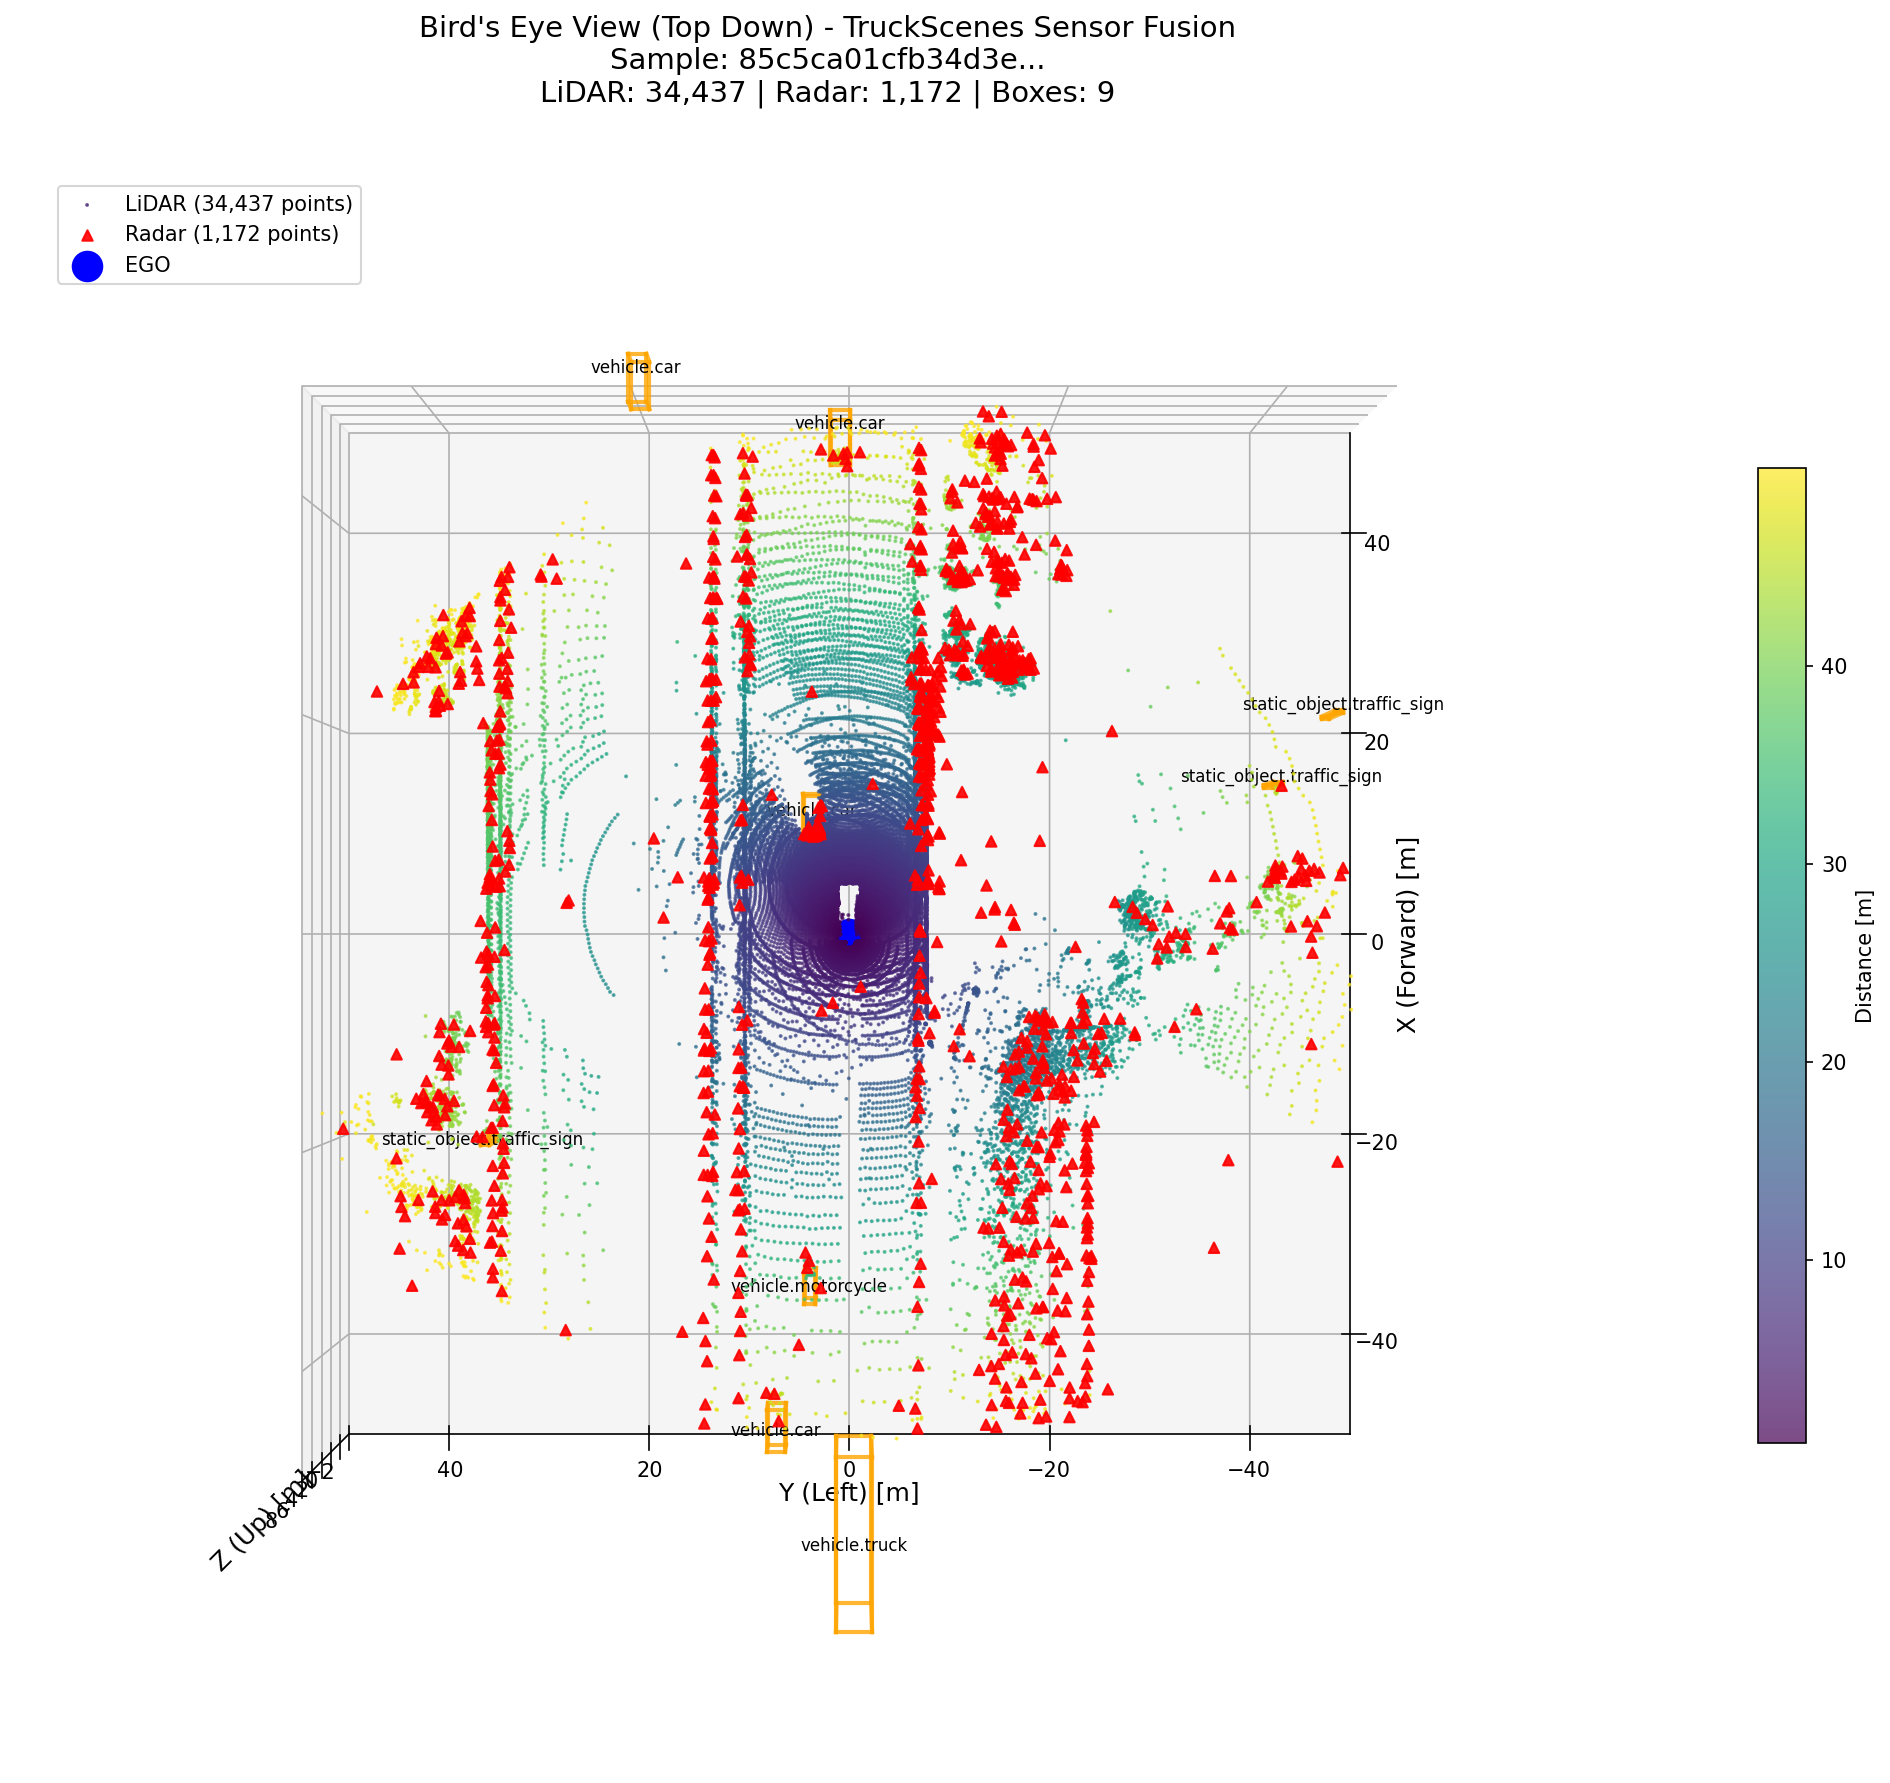
\includegraphics[height=4cm]{../output/scene_night_highway/85c5ca01cfb34d3e92d1c0c265235d04/visualizations/top_view.png}
        \caption*{(a) Bird’s Eye View}
    \end{minipage}
    % Side
    \begin{minipage}[t]{0.32\textwidth}
        \centering
        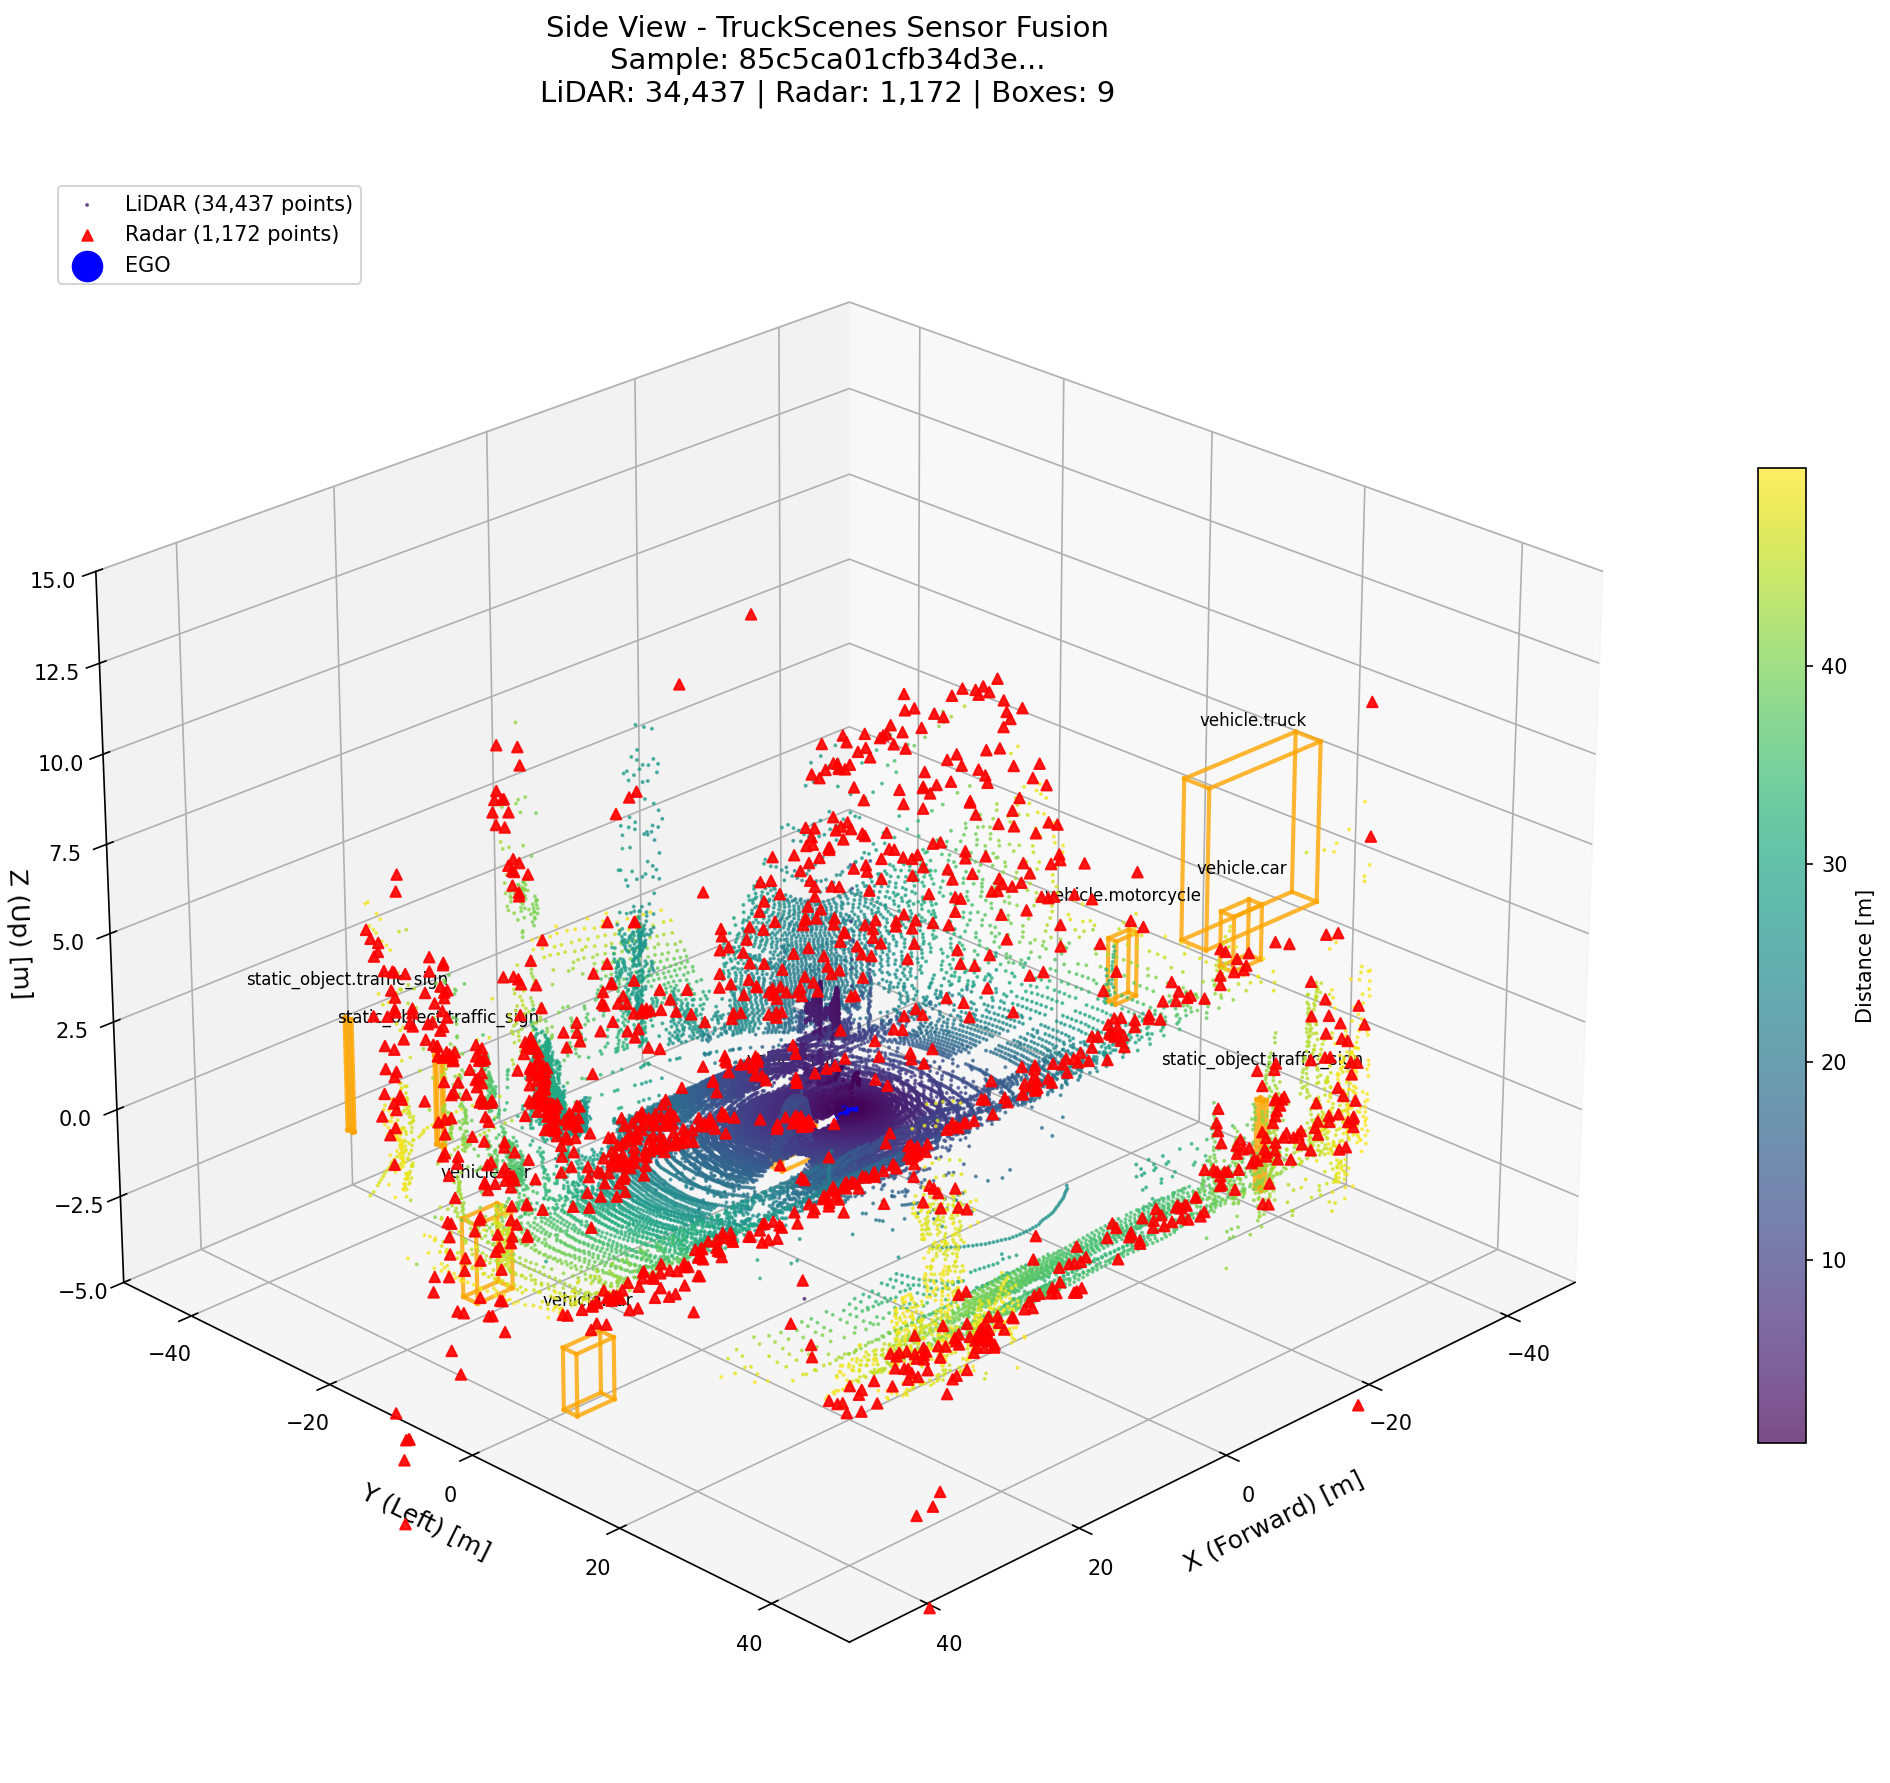
\includegraphics[height=4cm]{../output/scene_night_highway/85c5ca01cfb34d3e92d1c0c265235d04/visualizations/side_view.png}
        \caption*{(b) 3D Side View}
    \end{minipage}
    % Camera
    \begin{minipage}[t]{0.32\textwidth}
        \centering
        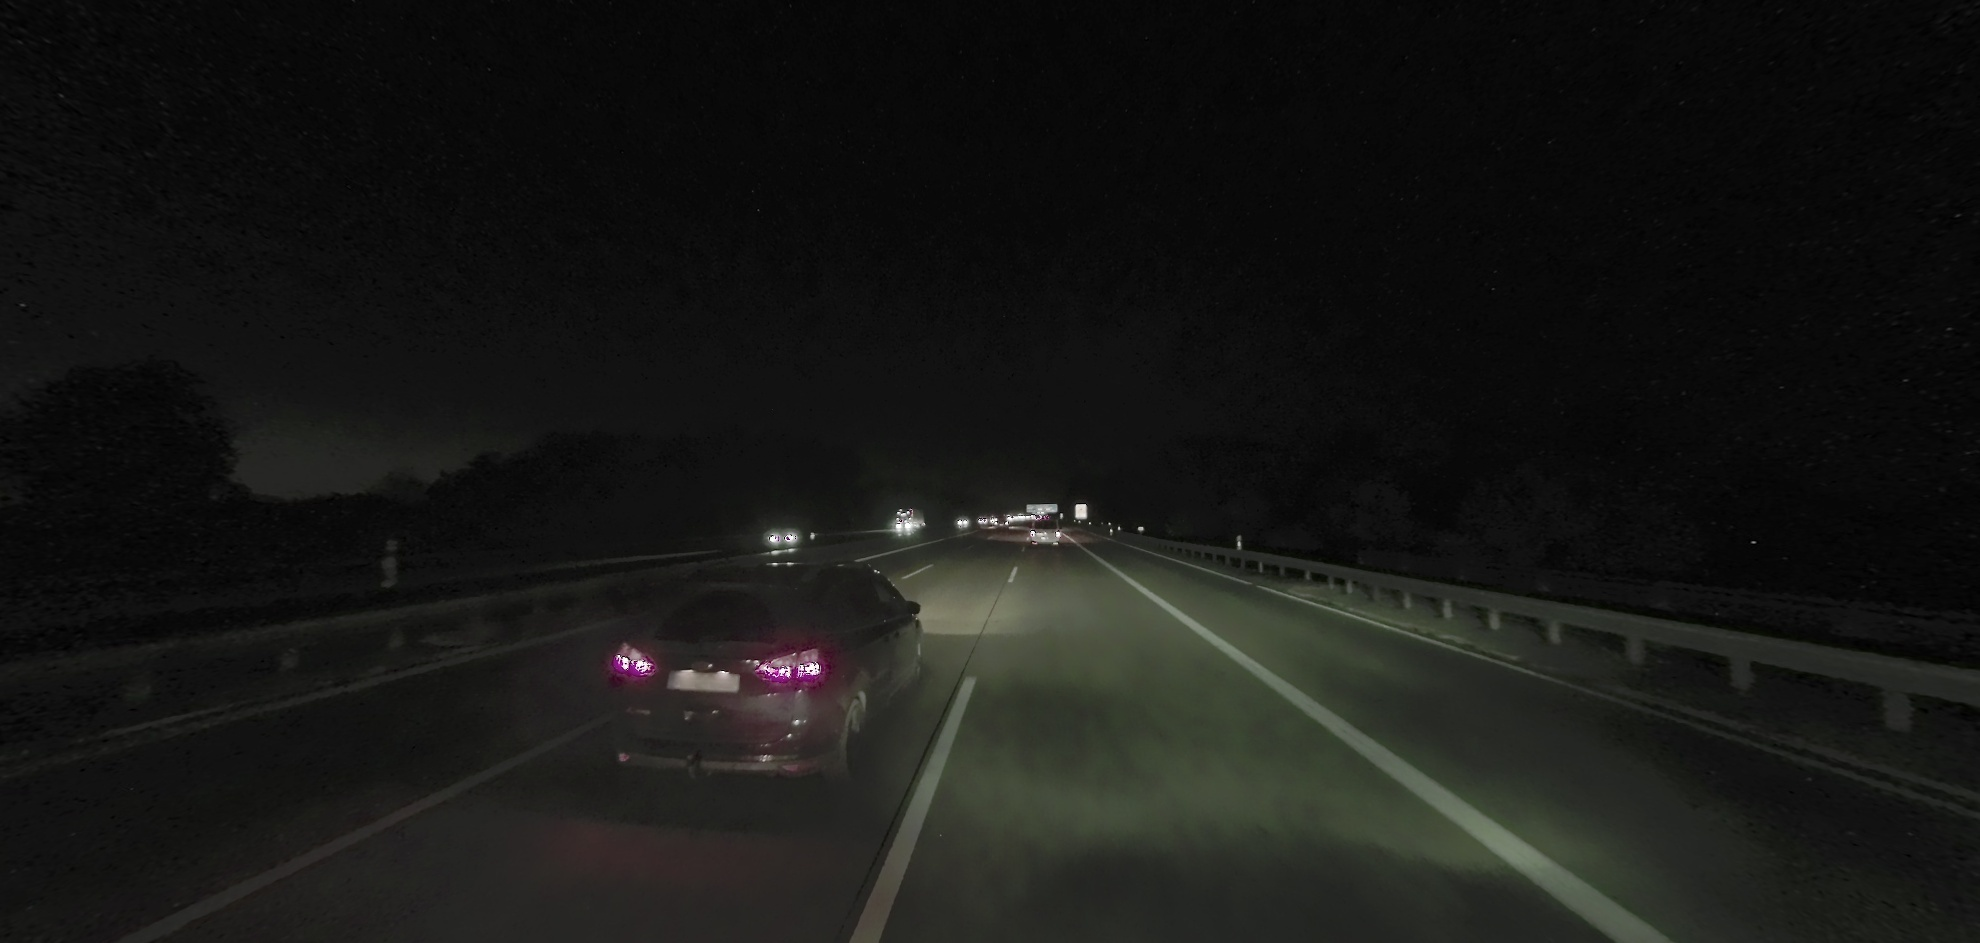
\includegraphics[height=2.9cm]{../output/scene_night_highway/85c5ca01cfb34d3e92d1c0c265235d04/front_left_camera.jpg}
        \caption*{(c) Front-left camera (driver)}
    \end{minipage}
    \caption{Visualization examples in the night highway scenario}
    \label{fig:night_highway_viz}
\end{figure}
In the night highway scenario, the fused point cloud achieves clear spatial coverage of distant vehicles and distant objects that are only sparsely represented or even missed by individual LiDAR or Radar. Occluded and low-reflectivity targets are reliably detected in the fusion result, demonstrating the necessity of multi-modal integration for night-time perception. The driver’s view confirms the presence of challenging, low-visibility targets which are successfully captured by sensor fusion.
% 或
For interactive 3D inspection, see the supplementary file:  \href{run:../output/scene_night_highway/85c5ca01cfb34d3e92d1c0c265235d04/interactive_3d.html}{night\_highway\_interactive\_3d.html}
\begin{small}
% 中文:夜间高速融合点云能显著提升远距离和低反射率目标的检测覆盖,单一传感器往往稀疏甚至漏检。融合结果补全了弱目标和遮挡目标,证明了夜间多模态感知的必要性。司机视角也验证了融合对低能见度目标的有效捕获。
\end{small}




\begin{figure}[H]
    \centering
    % BEV
    \begin{minipage}[t]{0.32\textwidth}
        \centering
        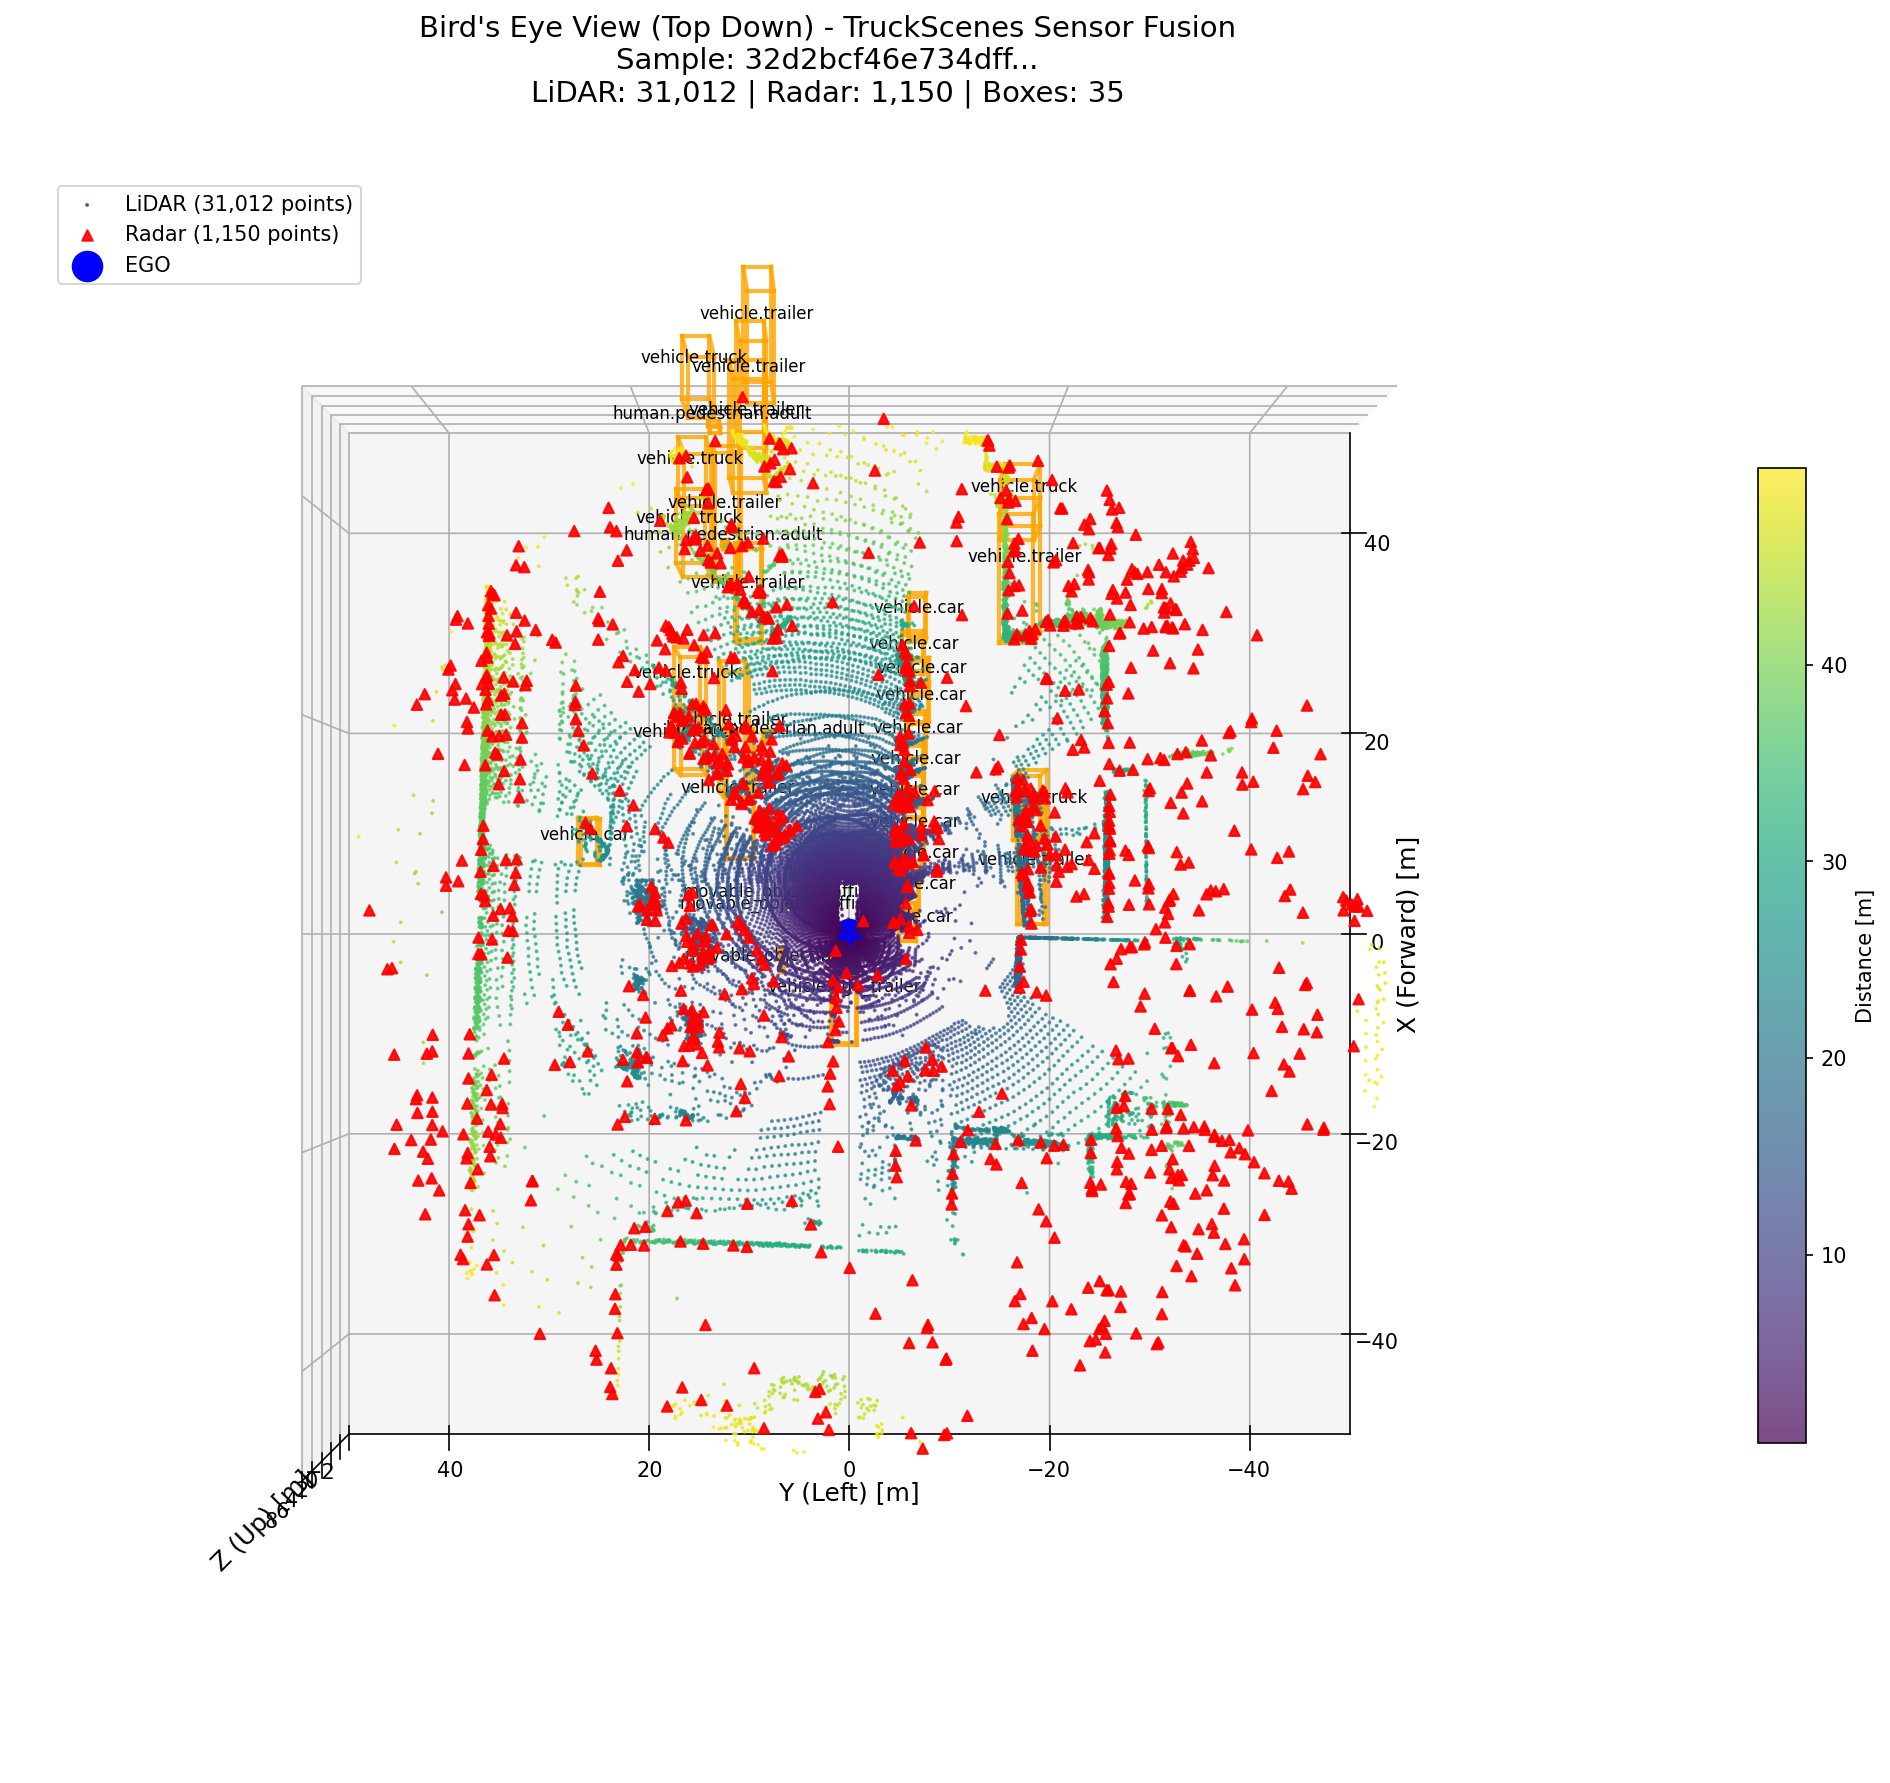
\includegraphics[height=4cm]{../output/scene_terminal_area/32d2bcf46e734dffb14fe2e0a823d059/visualizations/top_view.png}
        \caption*{(a) Bird’s Eye View}
    \end{minipage}
    % Side
    \begin{minipage}[t]{0.32\textwidth}
        \centering
        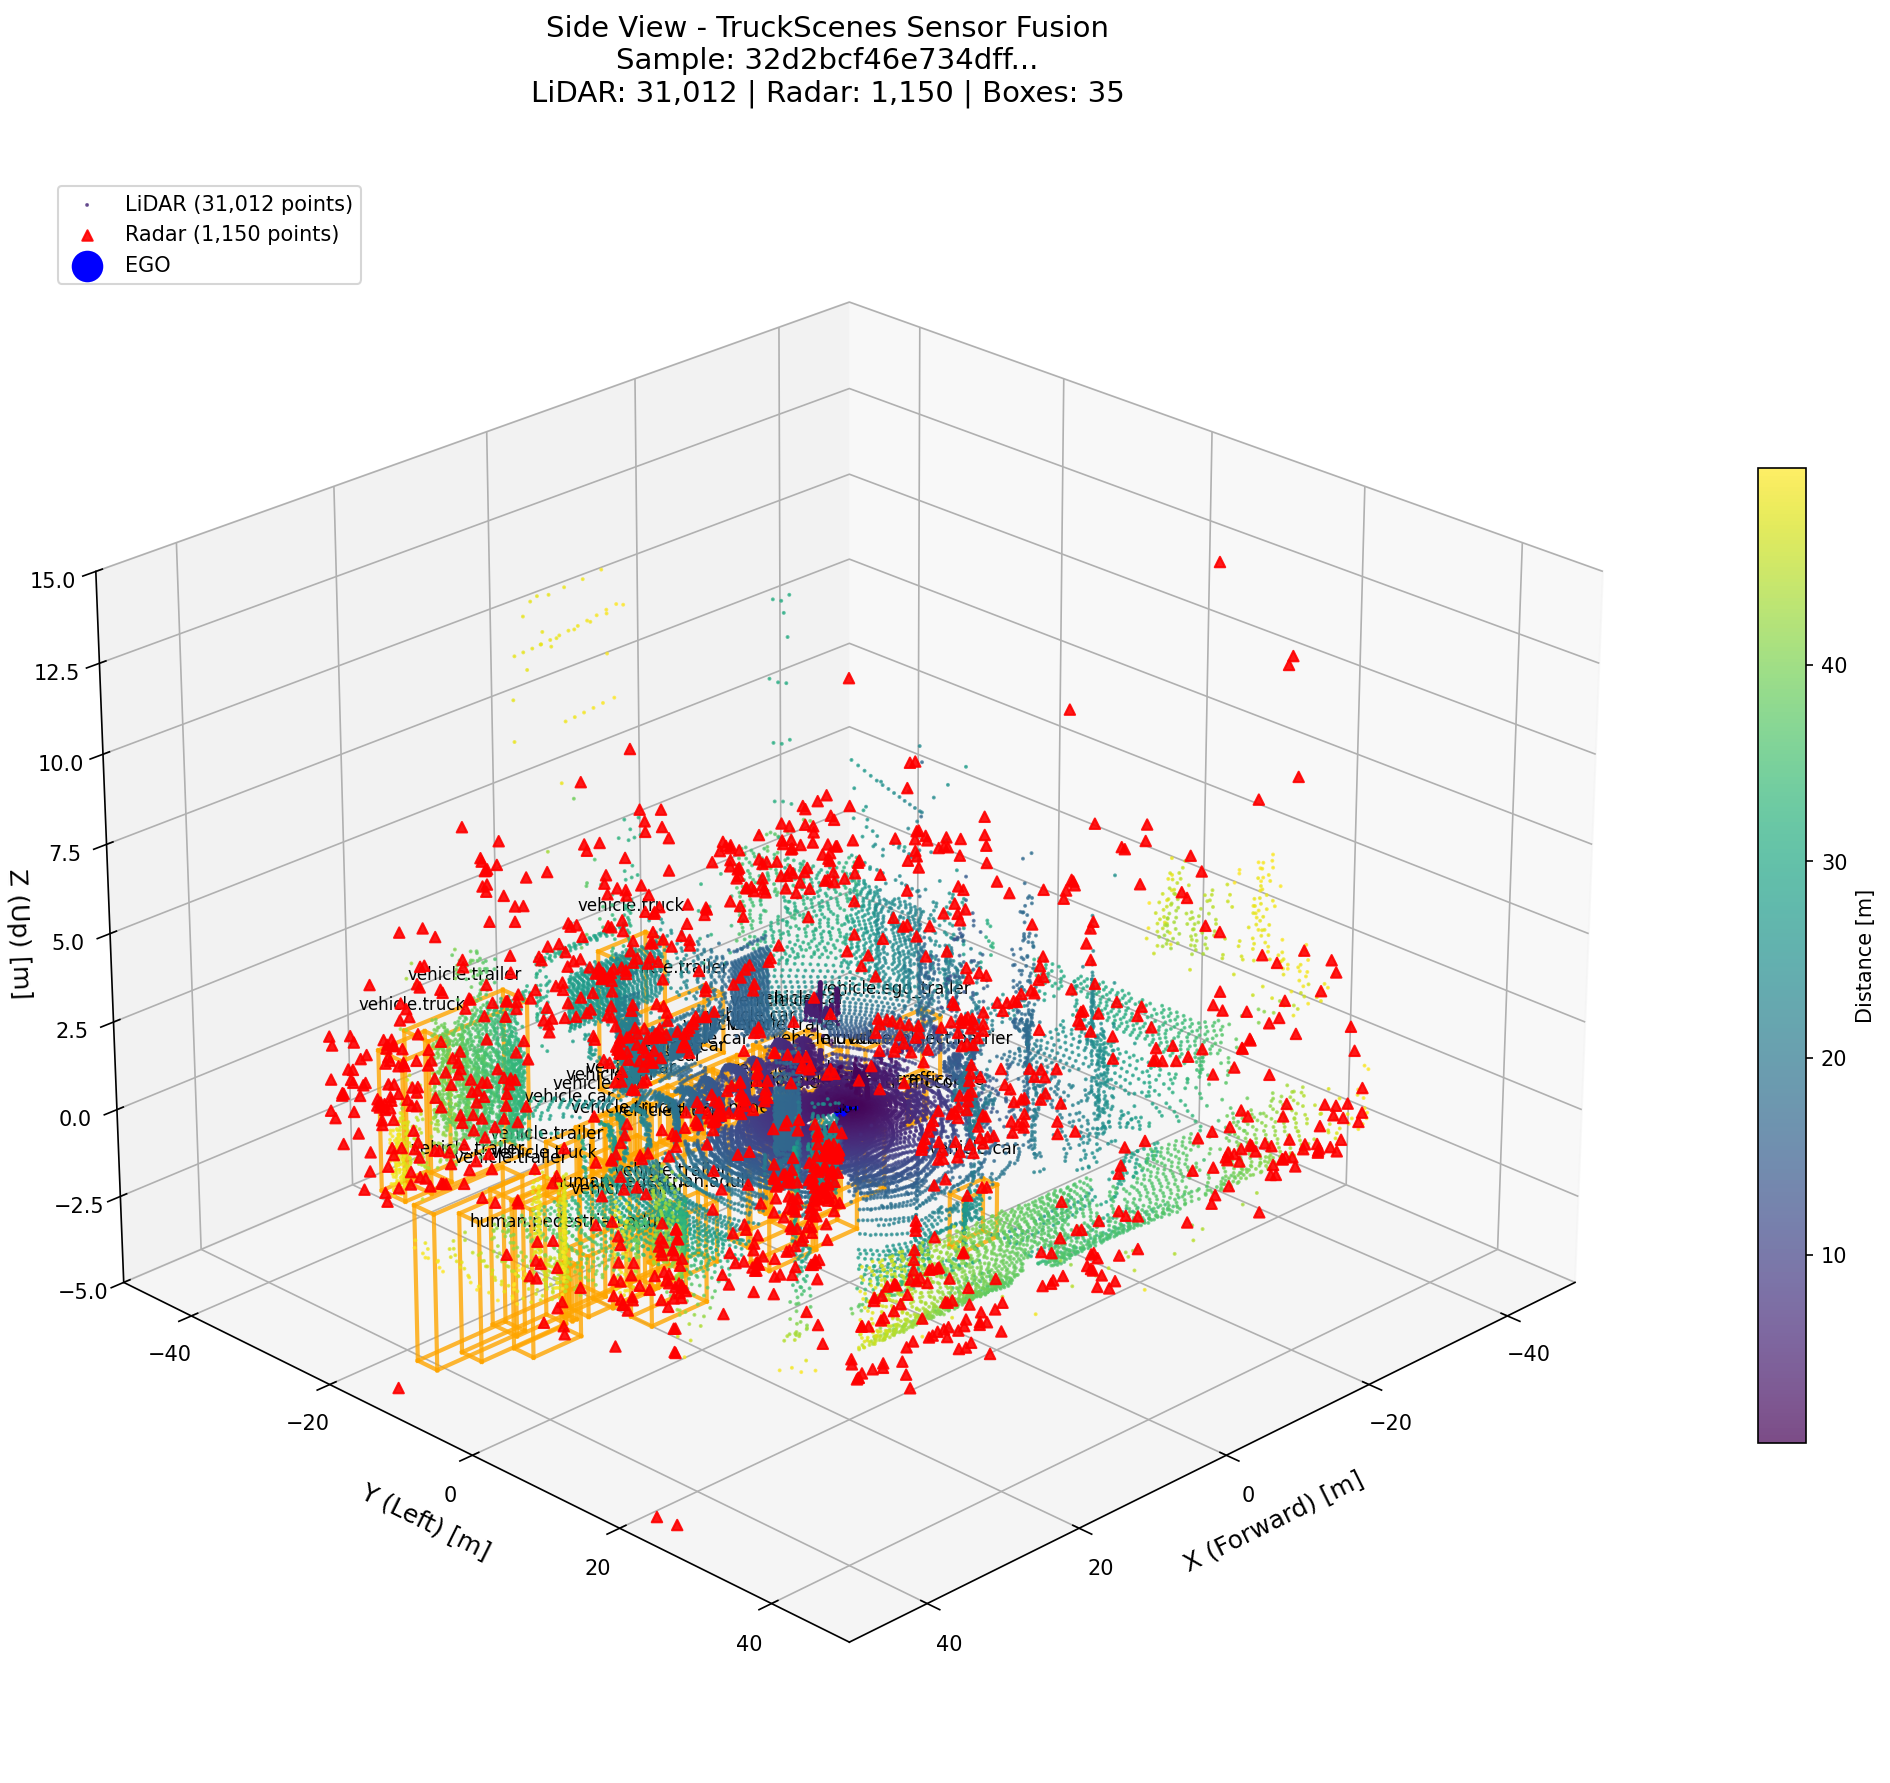
\includegraphics[height=4cm]{../output/scene_terminal_area/32d2bcf46e734dffb14fe2e0a823d059/visualizations/side_view.png}
        \caption*{(b) 3D Side View}
    \end{minipage}
    % Camera
    \begin{minipage}[t]{0.32\textwidth}
        \centering
        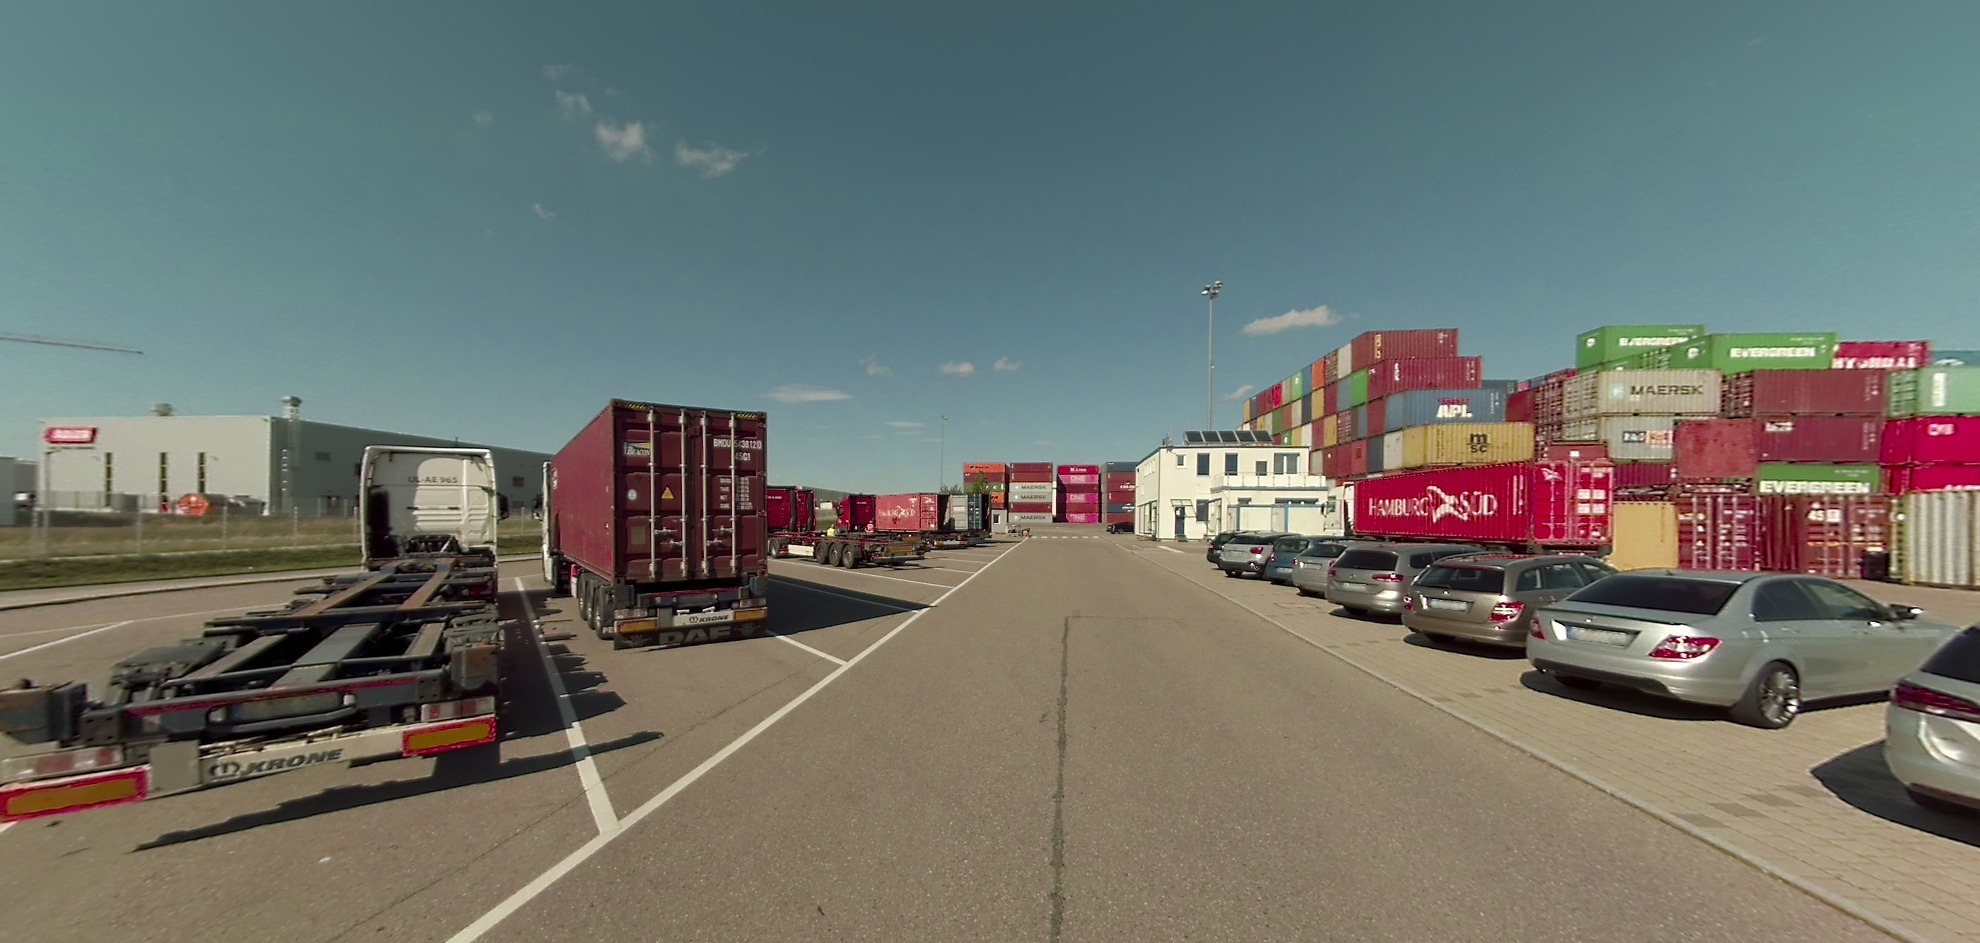
\includegraphics[height=2.9cm]{../output/scene_terminal_area/32d2bcf46e734dffb14fe2e0a823d059/front_left_camera.jpg}
        \caption*{(c) Front-left camera (driver)}
    \end{minipage}
    \caption{Visualization examples in the terminal area scenario}
    \label{fig:terminal_area_viz}
\end{figure}

In the terminal area scenario, dense occlusions and overlapping objects often lead to fragmented or missing detections when using a single sensor. Sensor fusion produces a more continuous and complete point cloud, enabling the restoration of partially occluded vehicles and static obstacles. The visualization shows that fusion outputs more coherent and spatially aligned bounding boxes compared to individual modalities.
For interactive 3D inspection, see the supplementary file:  \href{run:../output/scene_terminal_area/32d2bcf46e734dffb14fe2e0a823d059/interactive_3d.html}{terminal\_area\_interactive\_3d.html}
\begin{small}
% 中文:在物流终端场景中,密集遮挡和目标重叠容易导致单一传感器的检测碎片化或漏检。融合点云补全了部分遮挡车辆和静态障碍物,检测框更连续、空间对齐效果更好。
\end{small}


\begin{figure}[H]
	\centering
   % 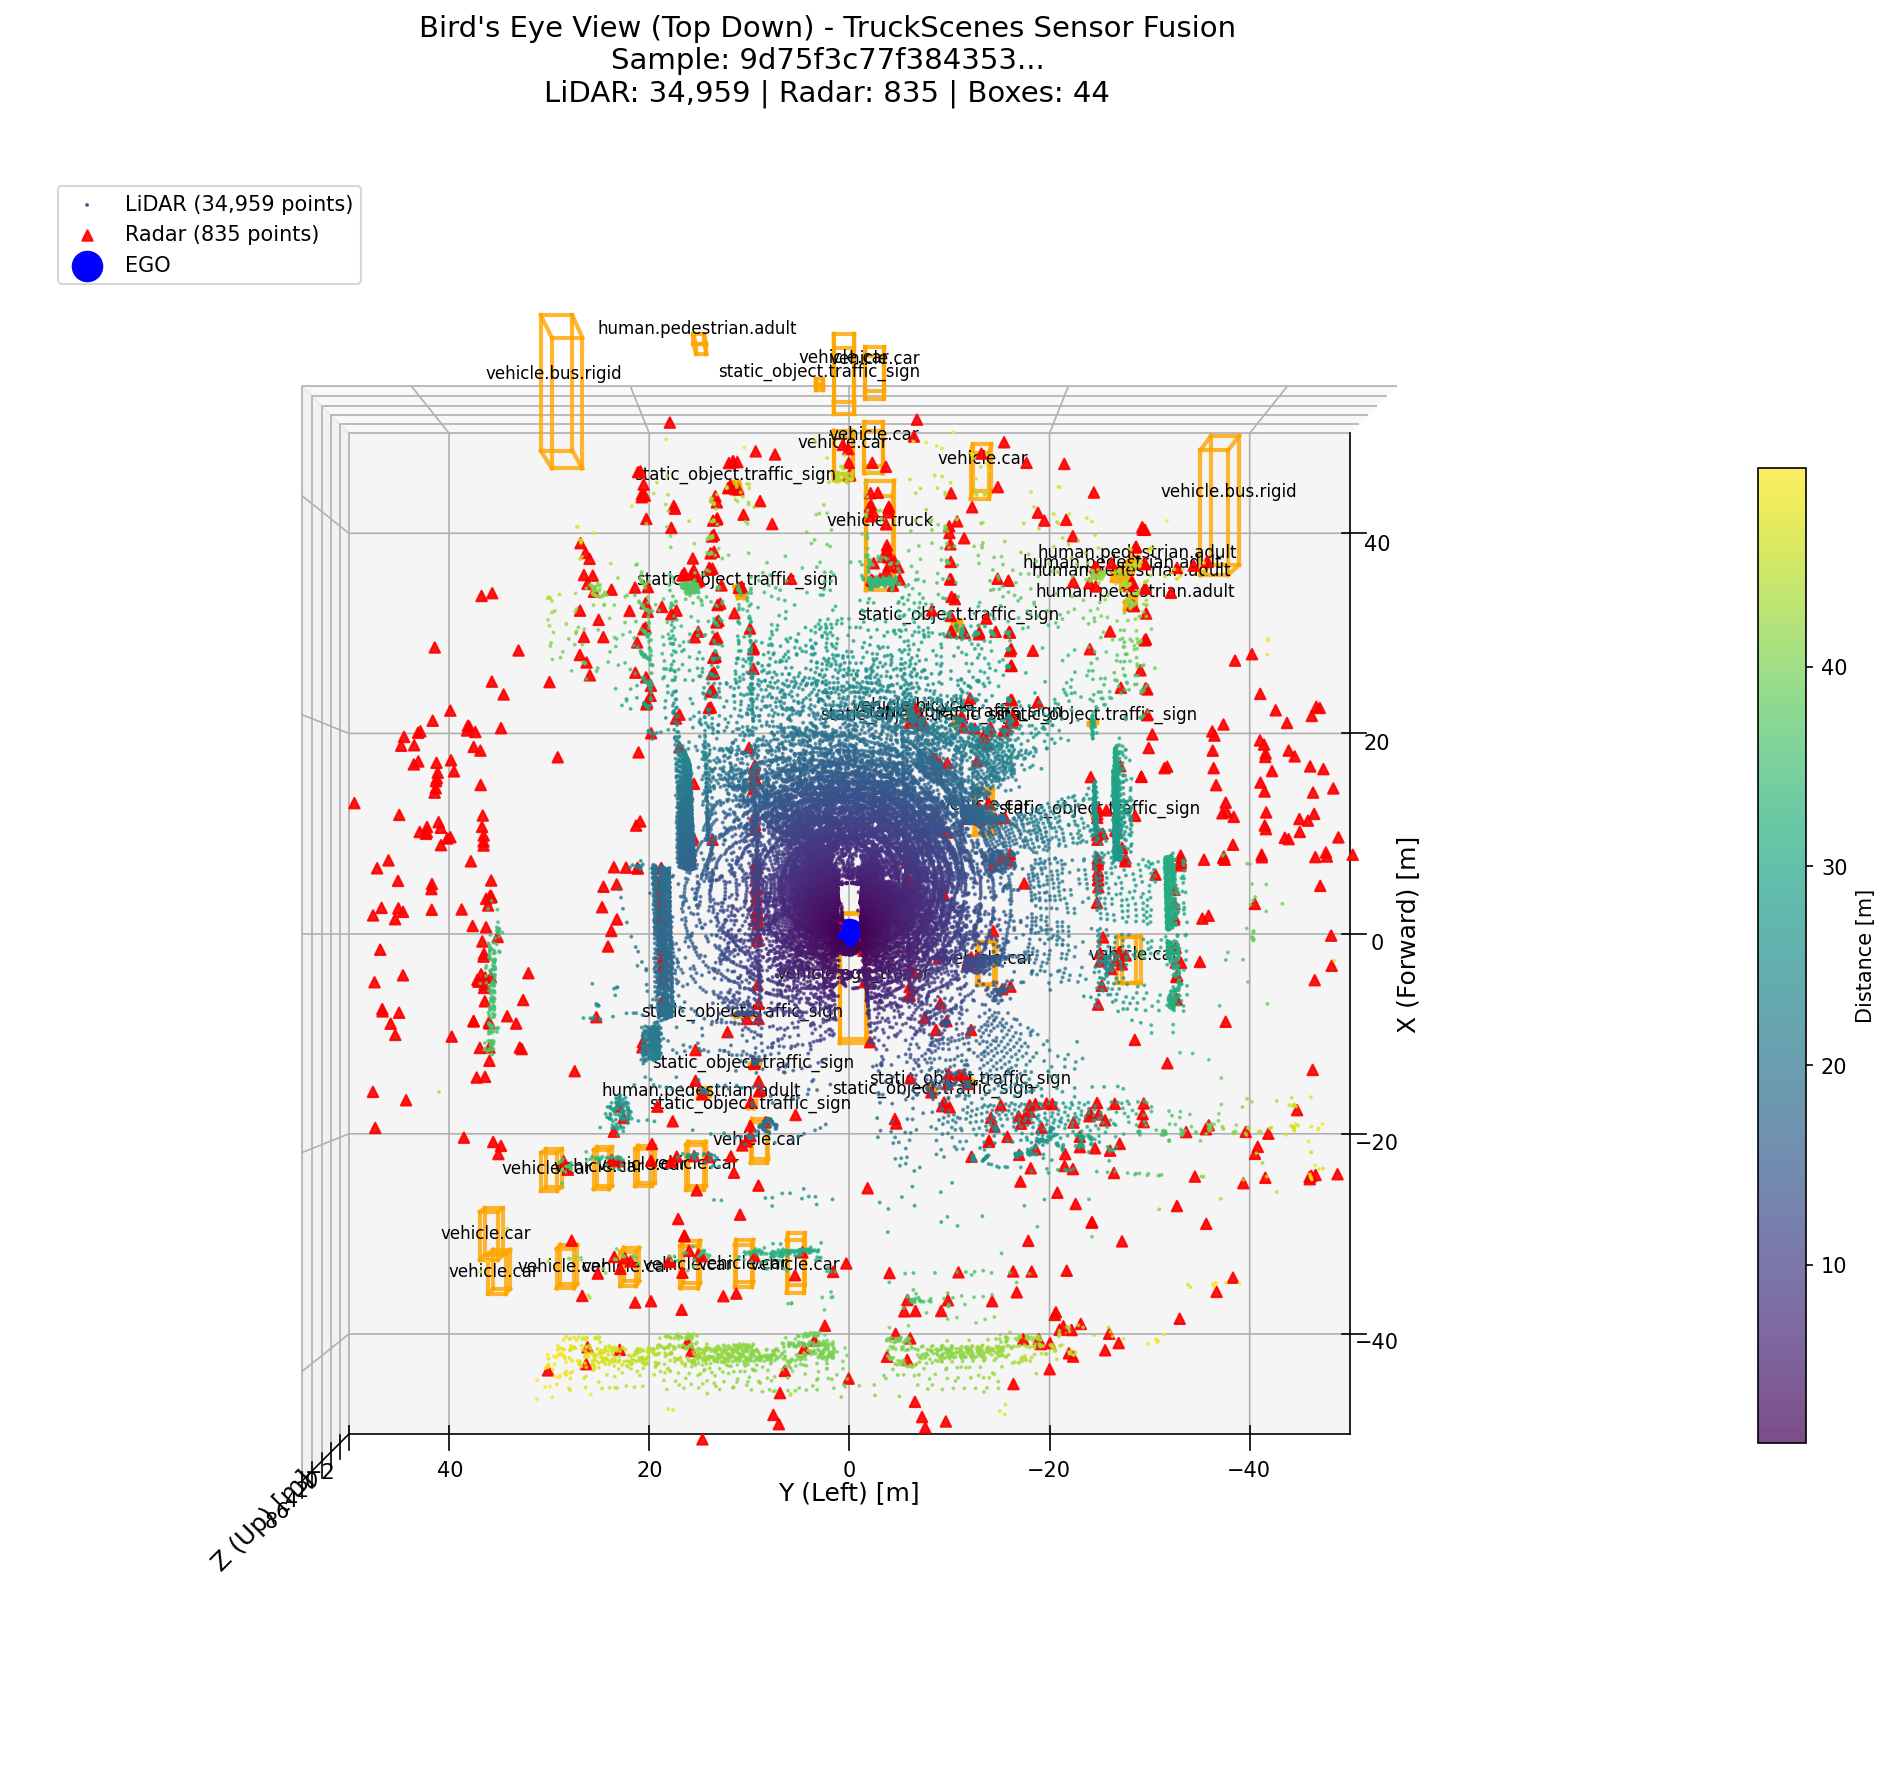
\includegraphics[width=0.32\textwidth]{top_view.png}
   % 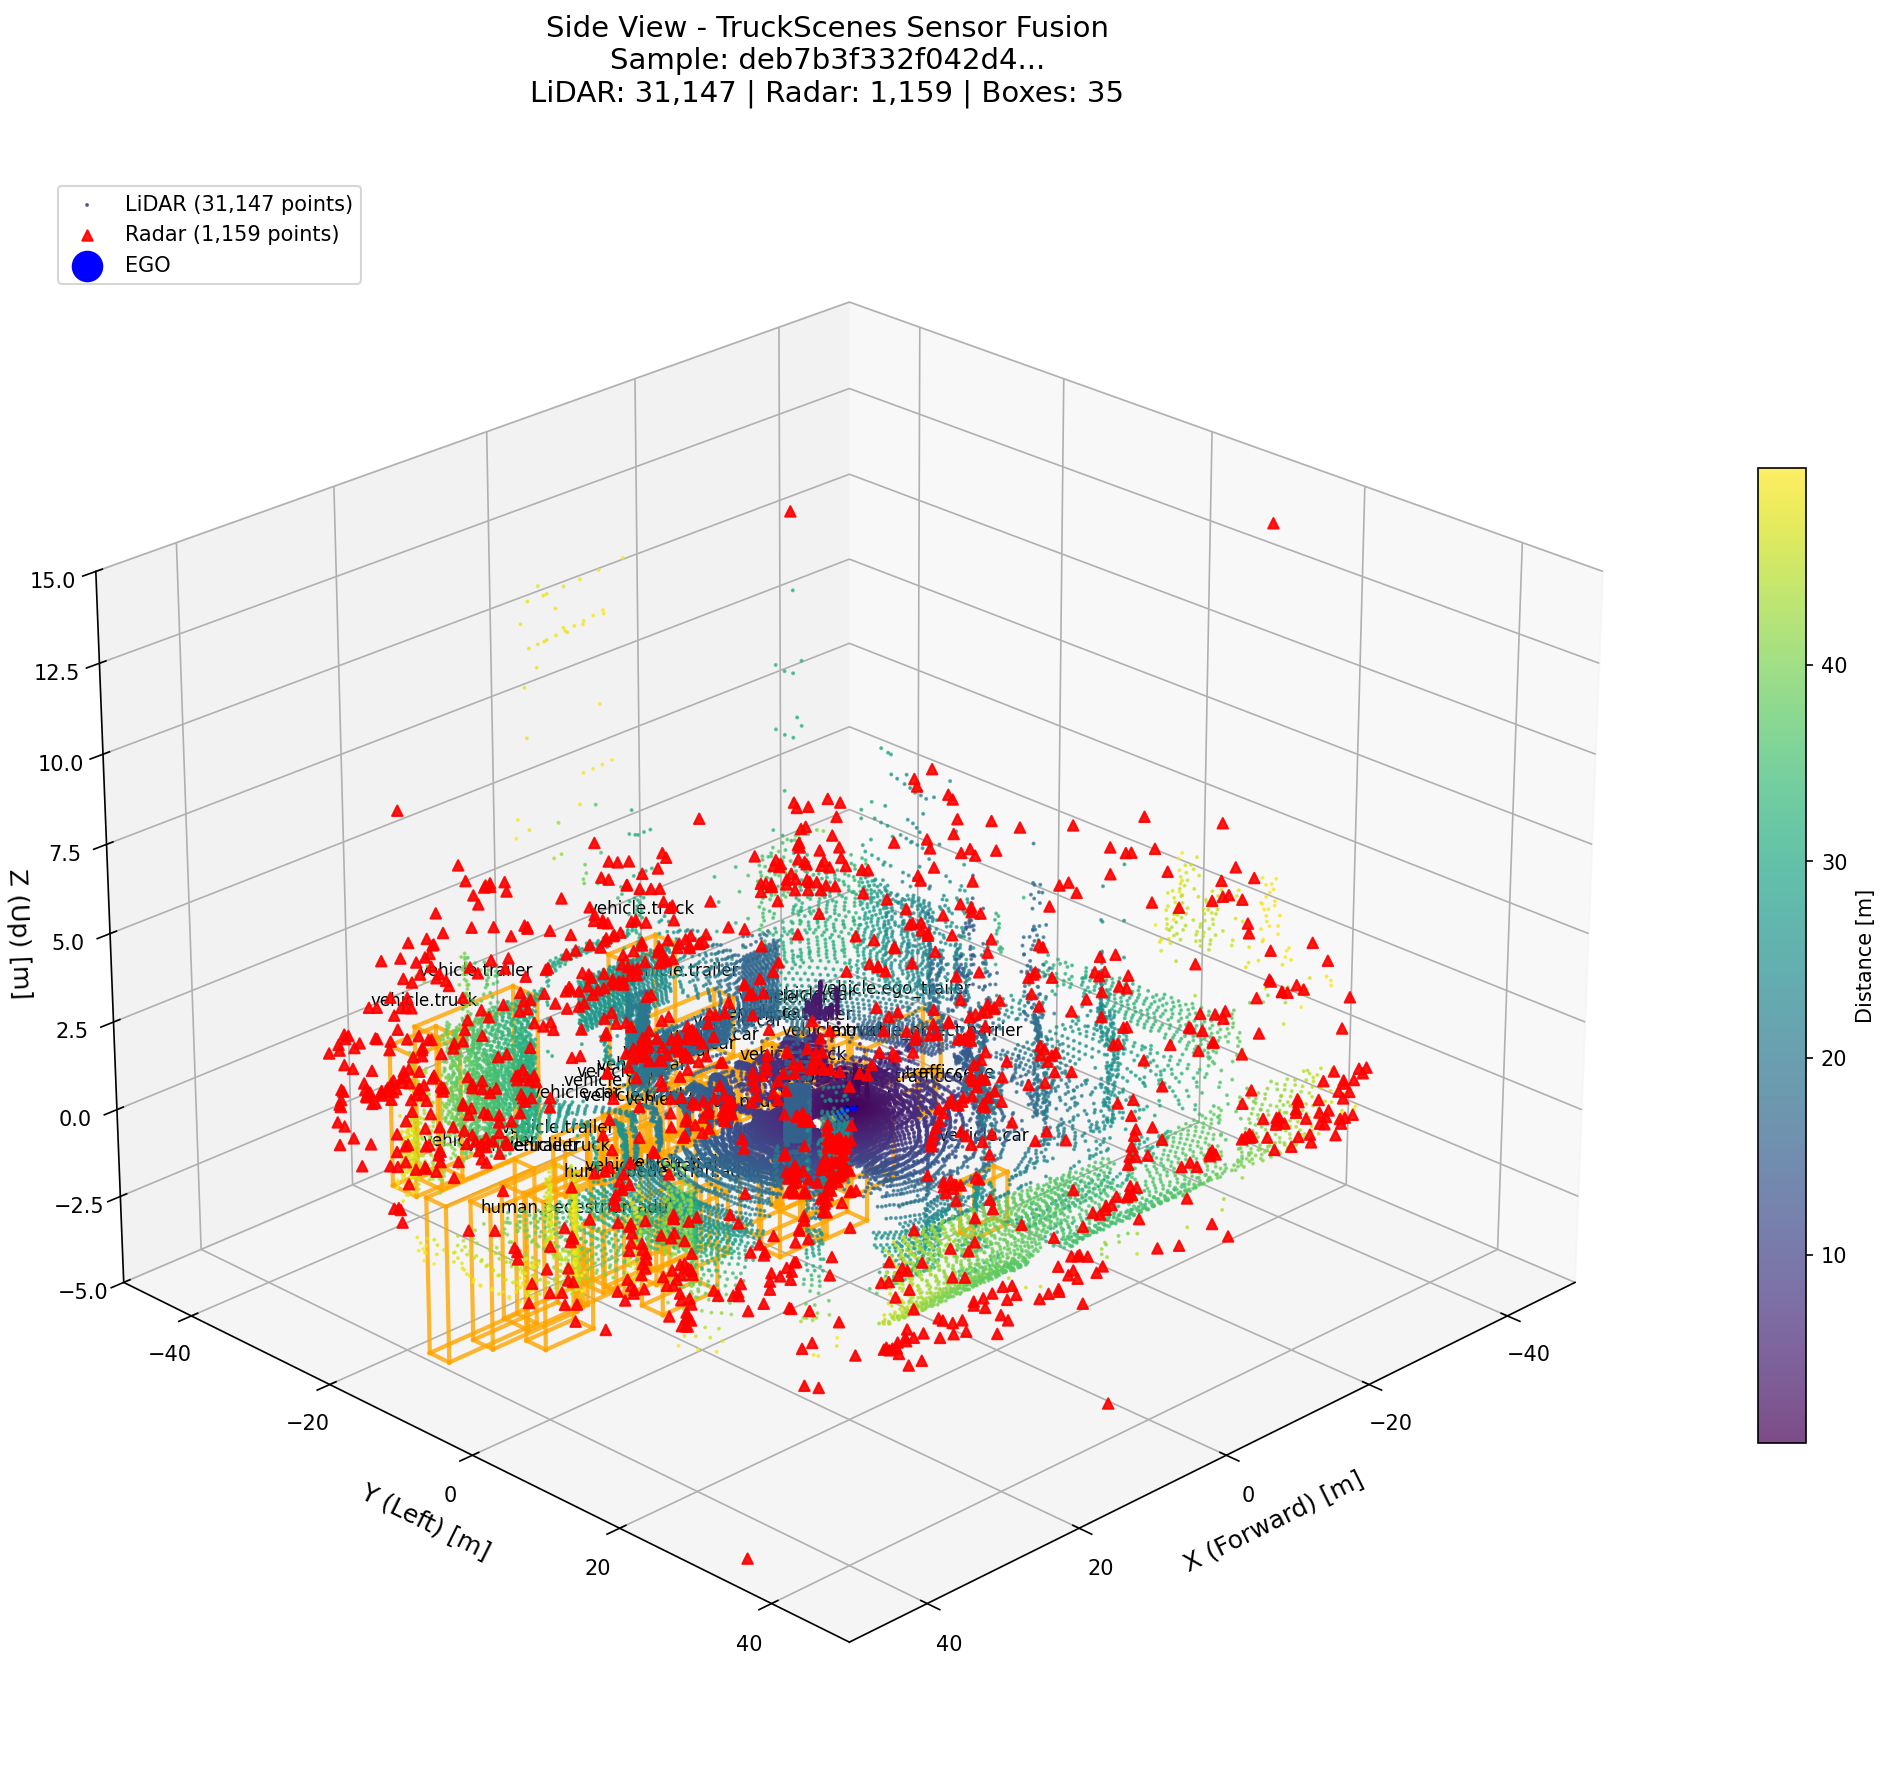
\includegraphics[width=0.32\textwidth]{side_view.png}
	%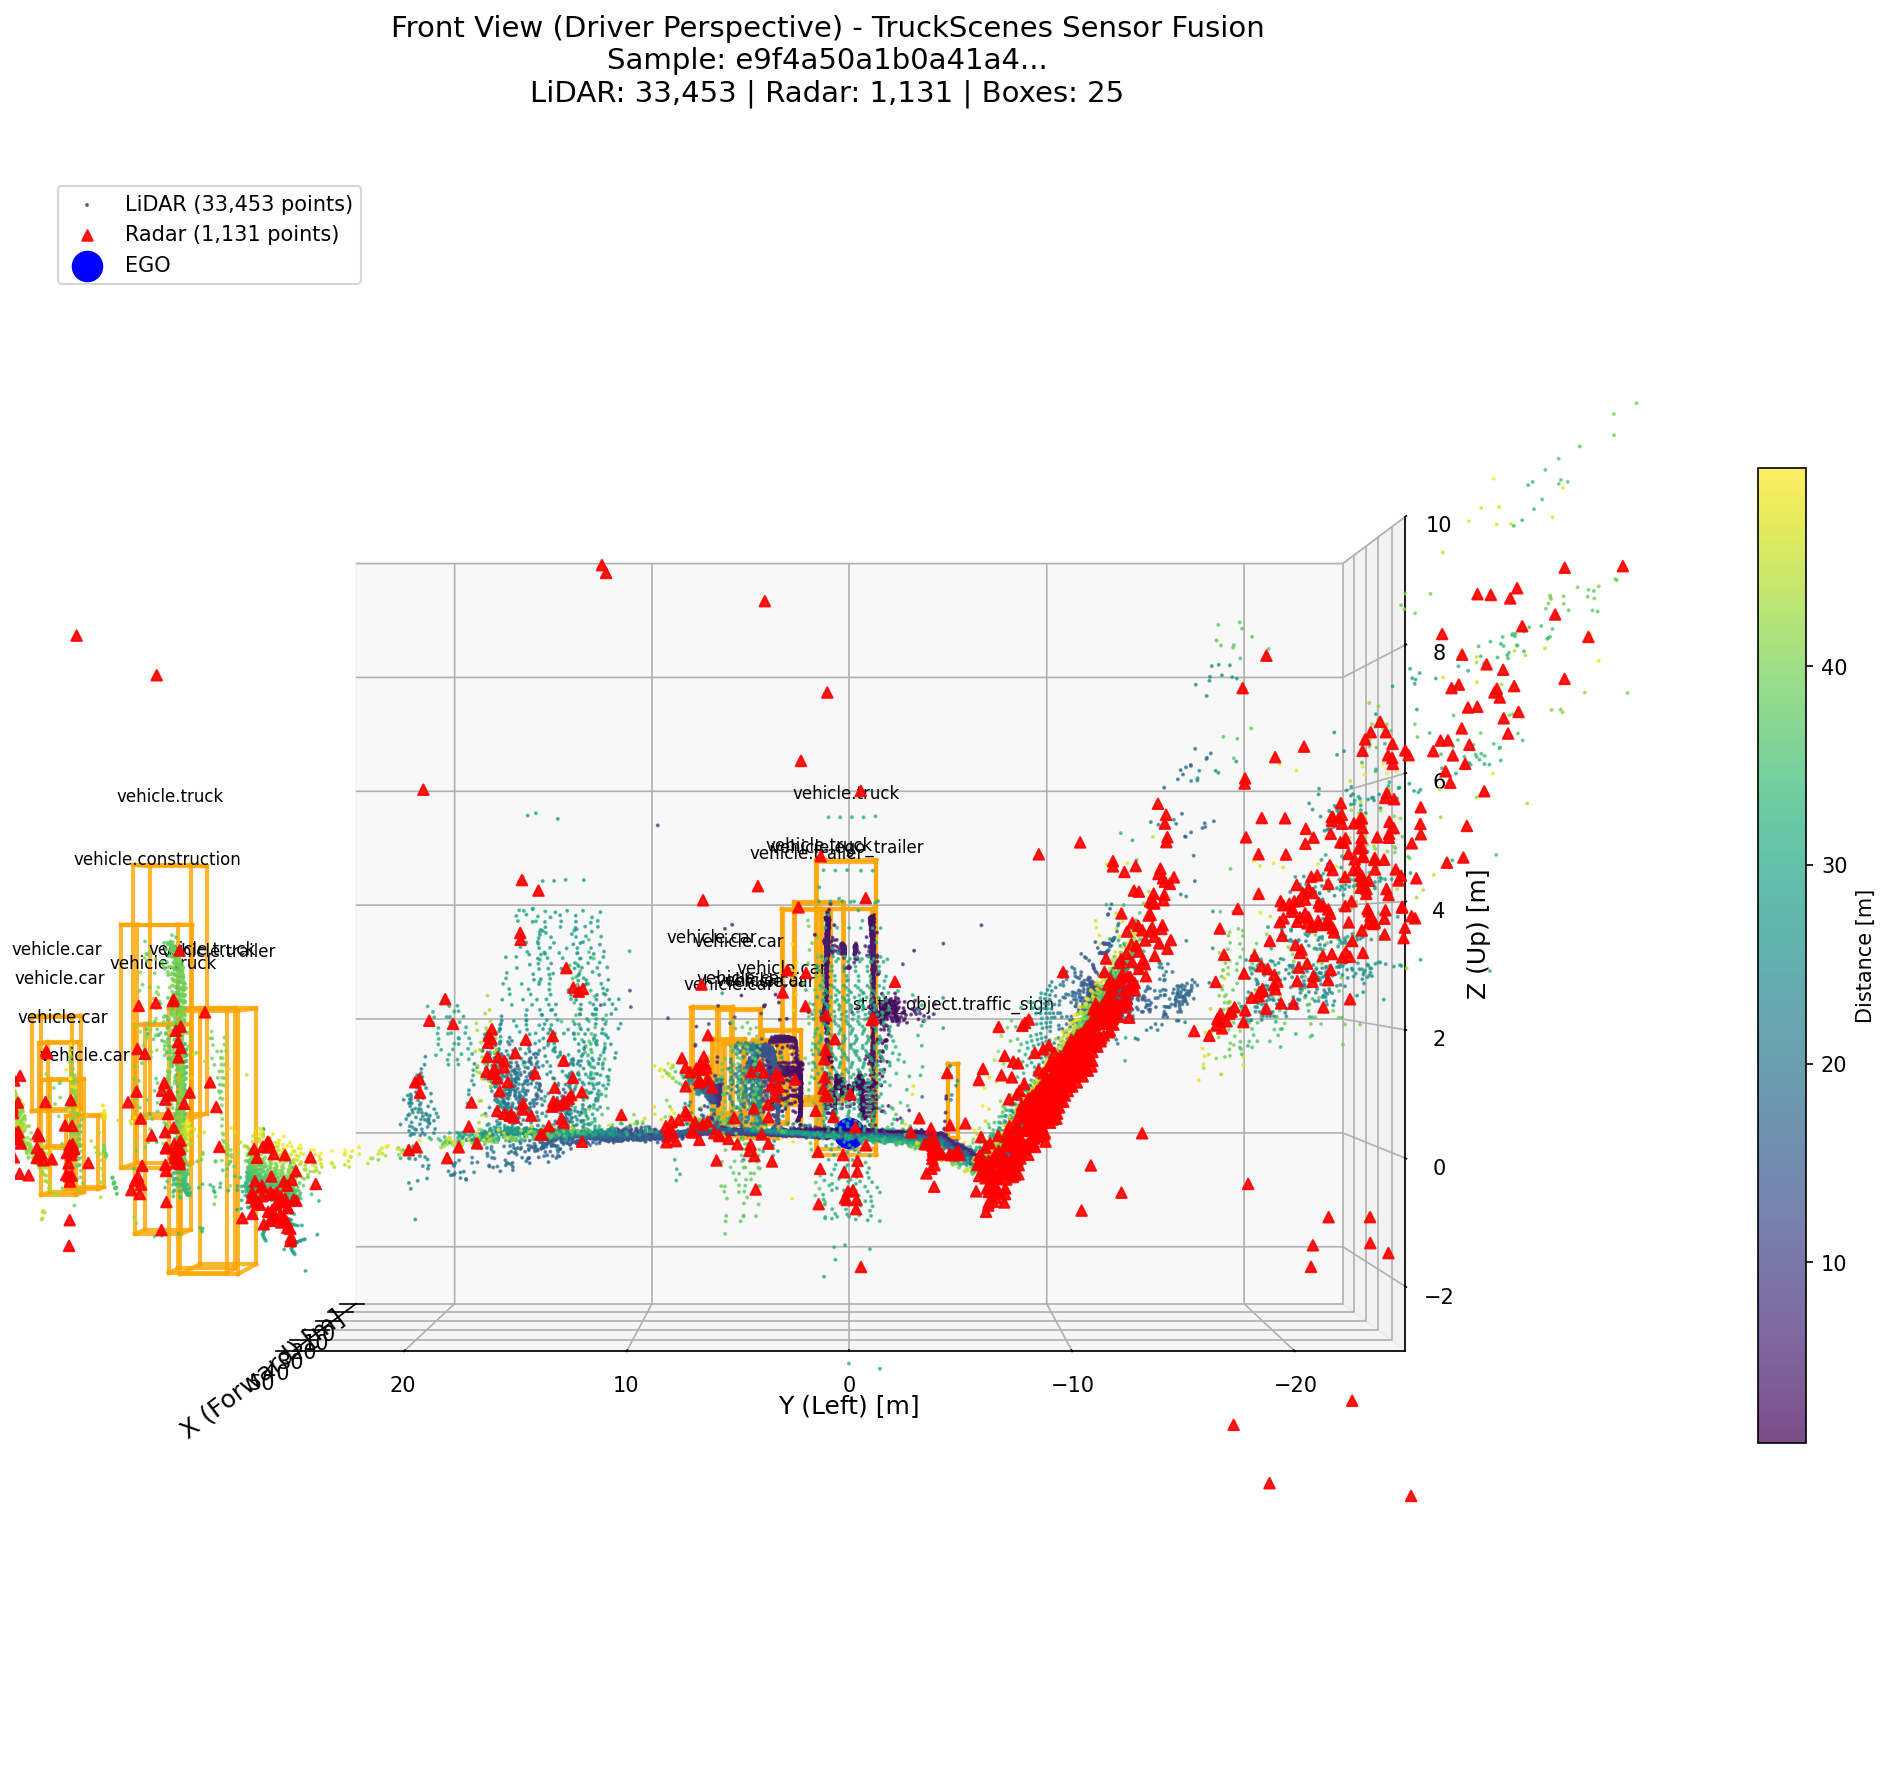
\includegraphics[width=0.32\textwidth]{front_view.png}
	%\caption{Sensor fusion point cloud visualizations: BEV (left), side view (center), and front view (right), with overlaid 3D bounding boxes.}
   % \label{fig:3d_bev}
\end{figure}

\subsection{Scenario-Based Performance}
Detection recall for each sensor modality and the fused result has been assessed under various driving scenes. As shown in Figure~\ref{fig:recall_by_scene}, sensor fusion consistently achieves higher recall rates than any single modality, particularly in challenging conditions such as nighttime or adverse weather.

\begin{figure}[H]
    \centering
    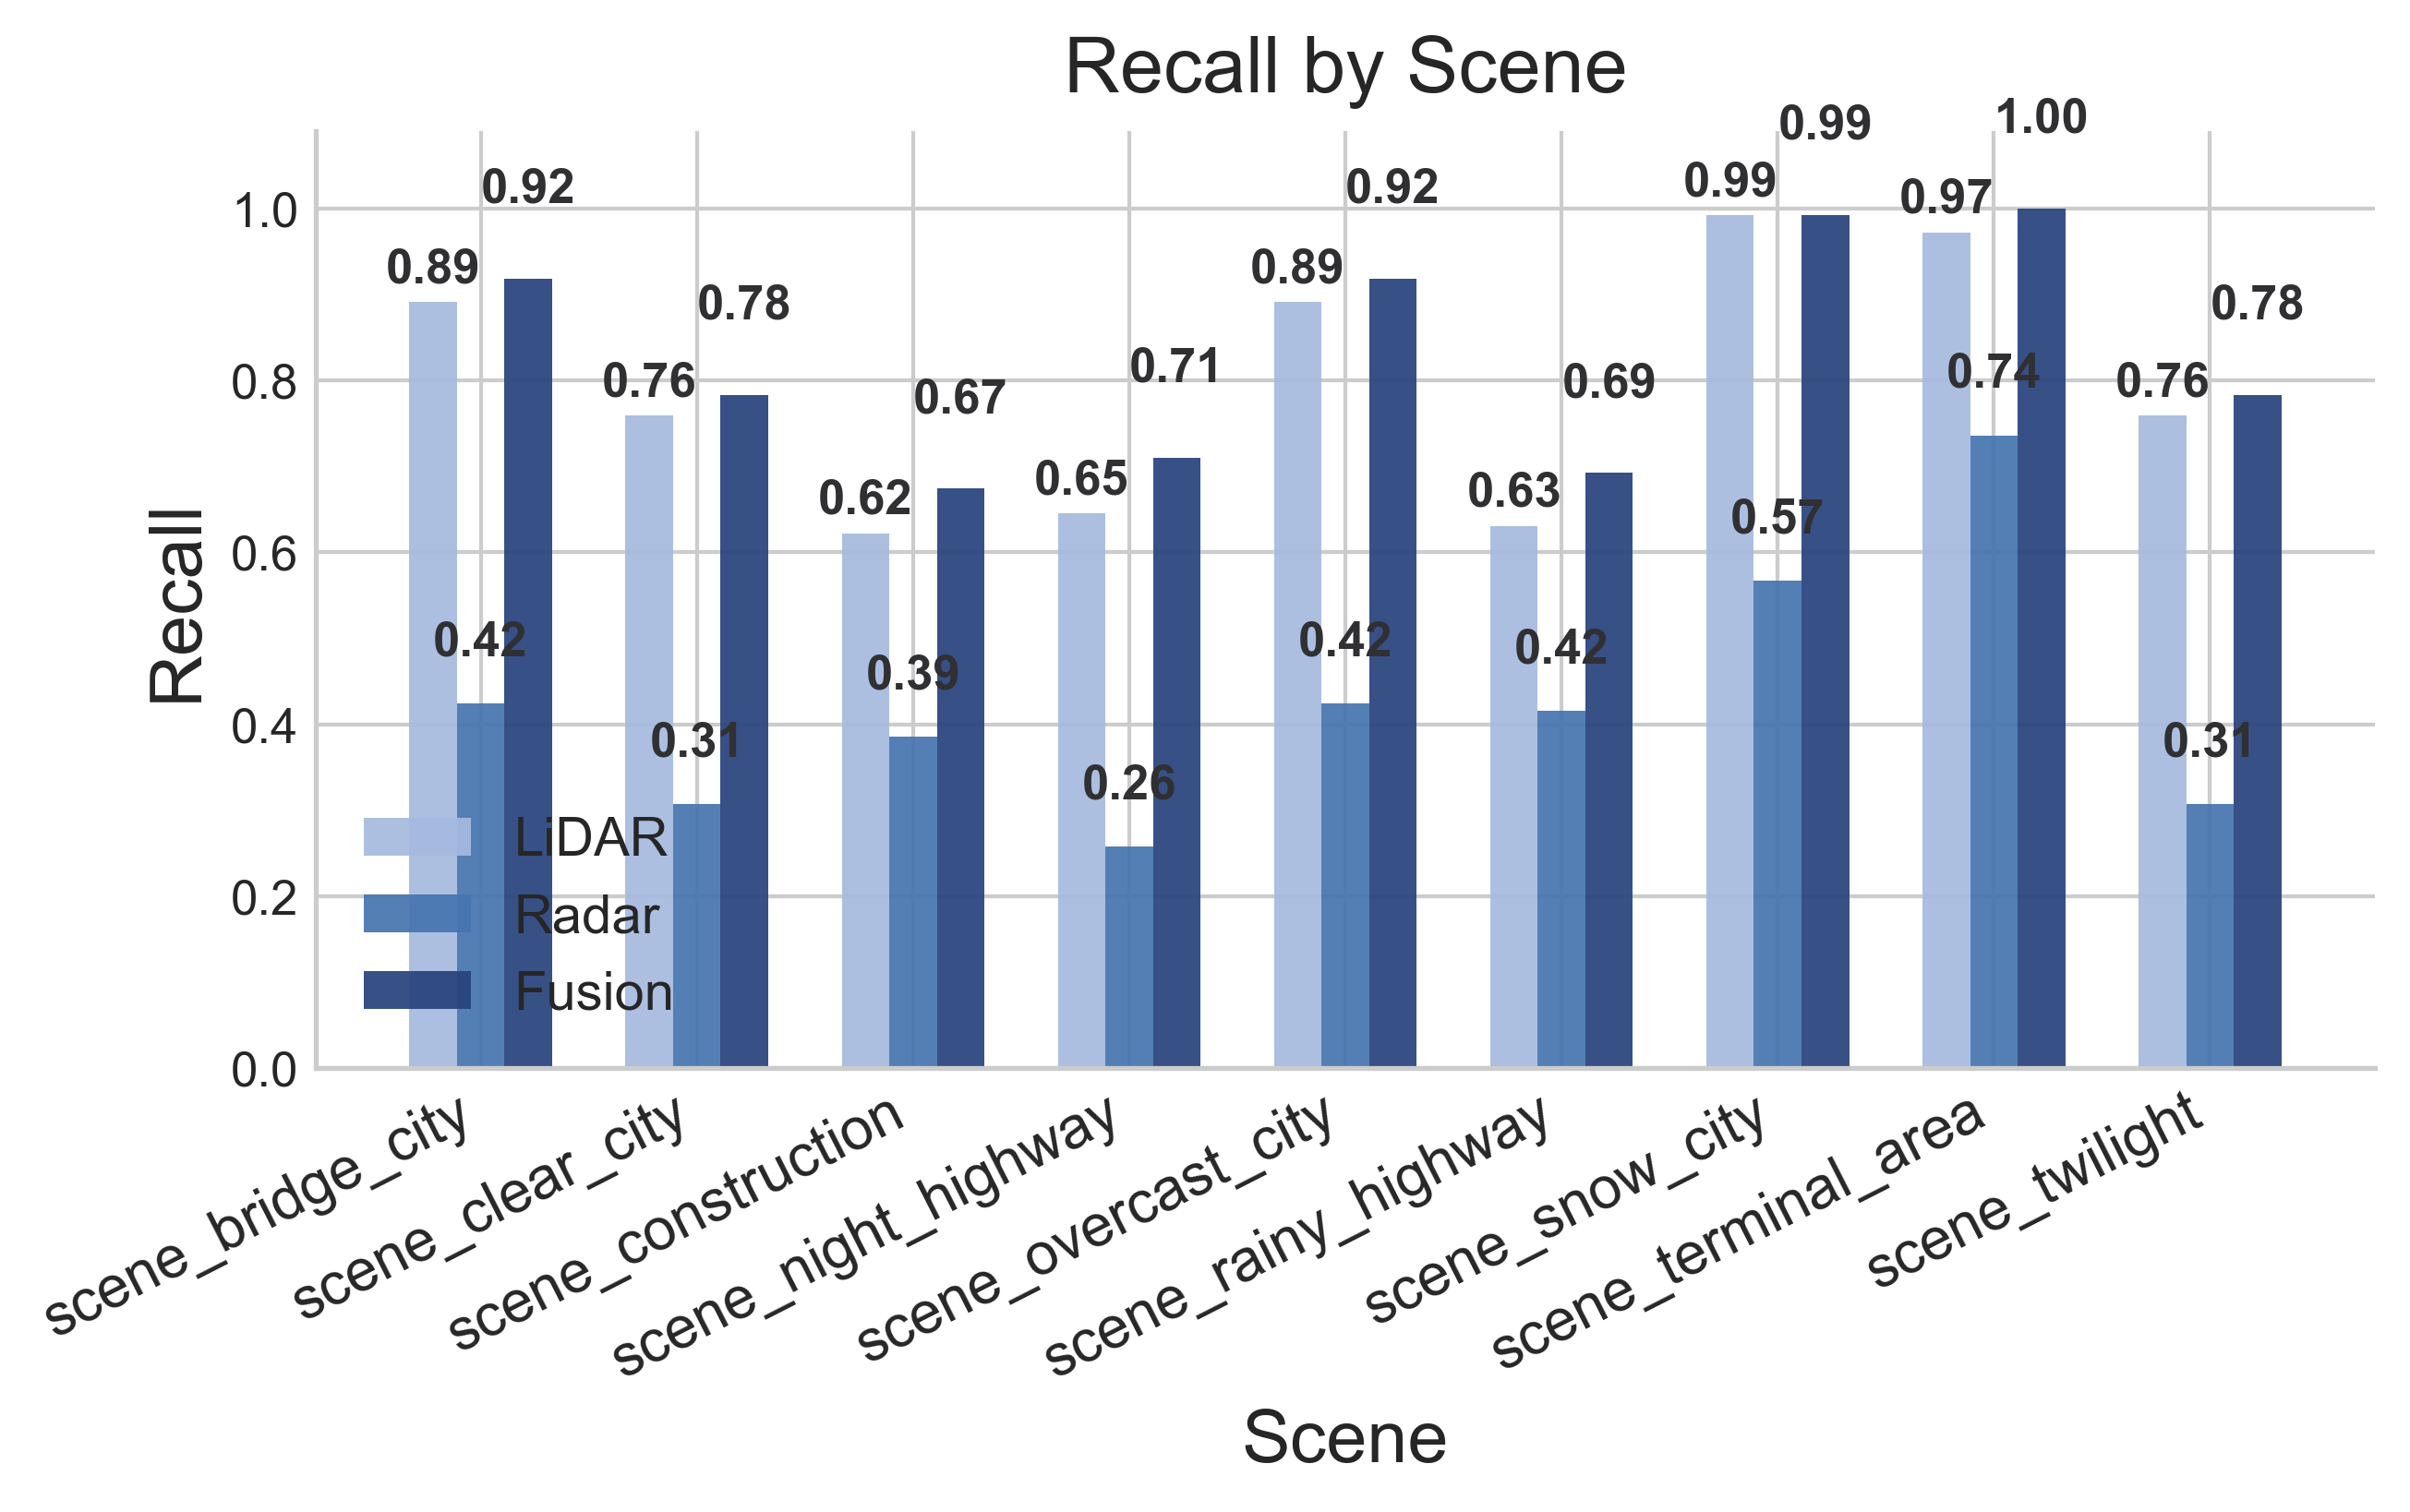
\includegraphics[width=0.7\textwidth]{../output/plots/recall_by_scene.png}
    \caption{Detection recall by scenario.}
    \label{fig:recall_by_scene}
\end{figure}

\begin{small}
% 中文:在不同驾驶场景下评估各模态与融合的检测recall。如图\ref{fig:recall_by_scene}所示,融合检测在夜间及复杂天气下表现尤为突出。
\end{small}


\subsection{Category-Wise Analysis}
Recall by object category is visualized in Figure~\ref{fig:recall_by_category}. Superior performance from sensor fusion is observed for most categories, with significant gains for vulnerable road users (e.g., pedestrians, cyclists) and certain vehicle types. This demonstrates the complementary advantages of multi-sensor integration.

\begin{figure}[H]
    \centering
    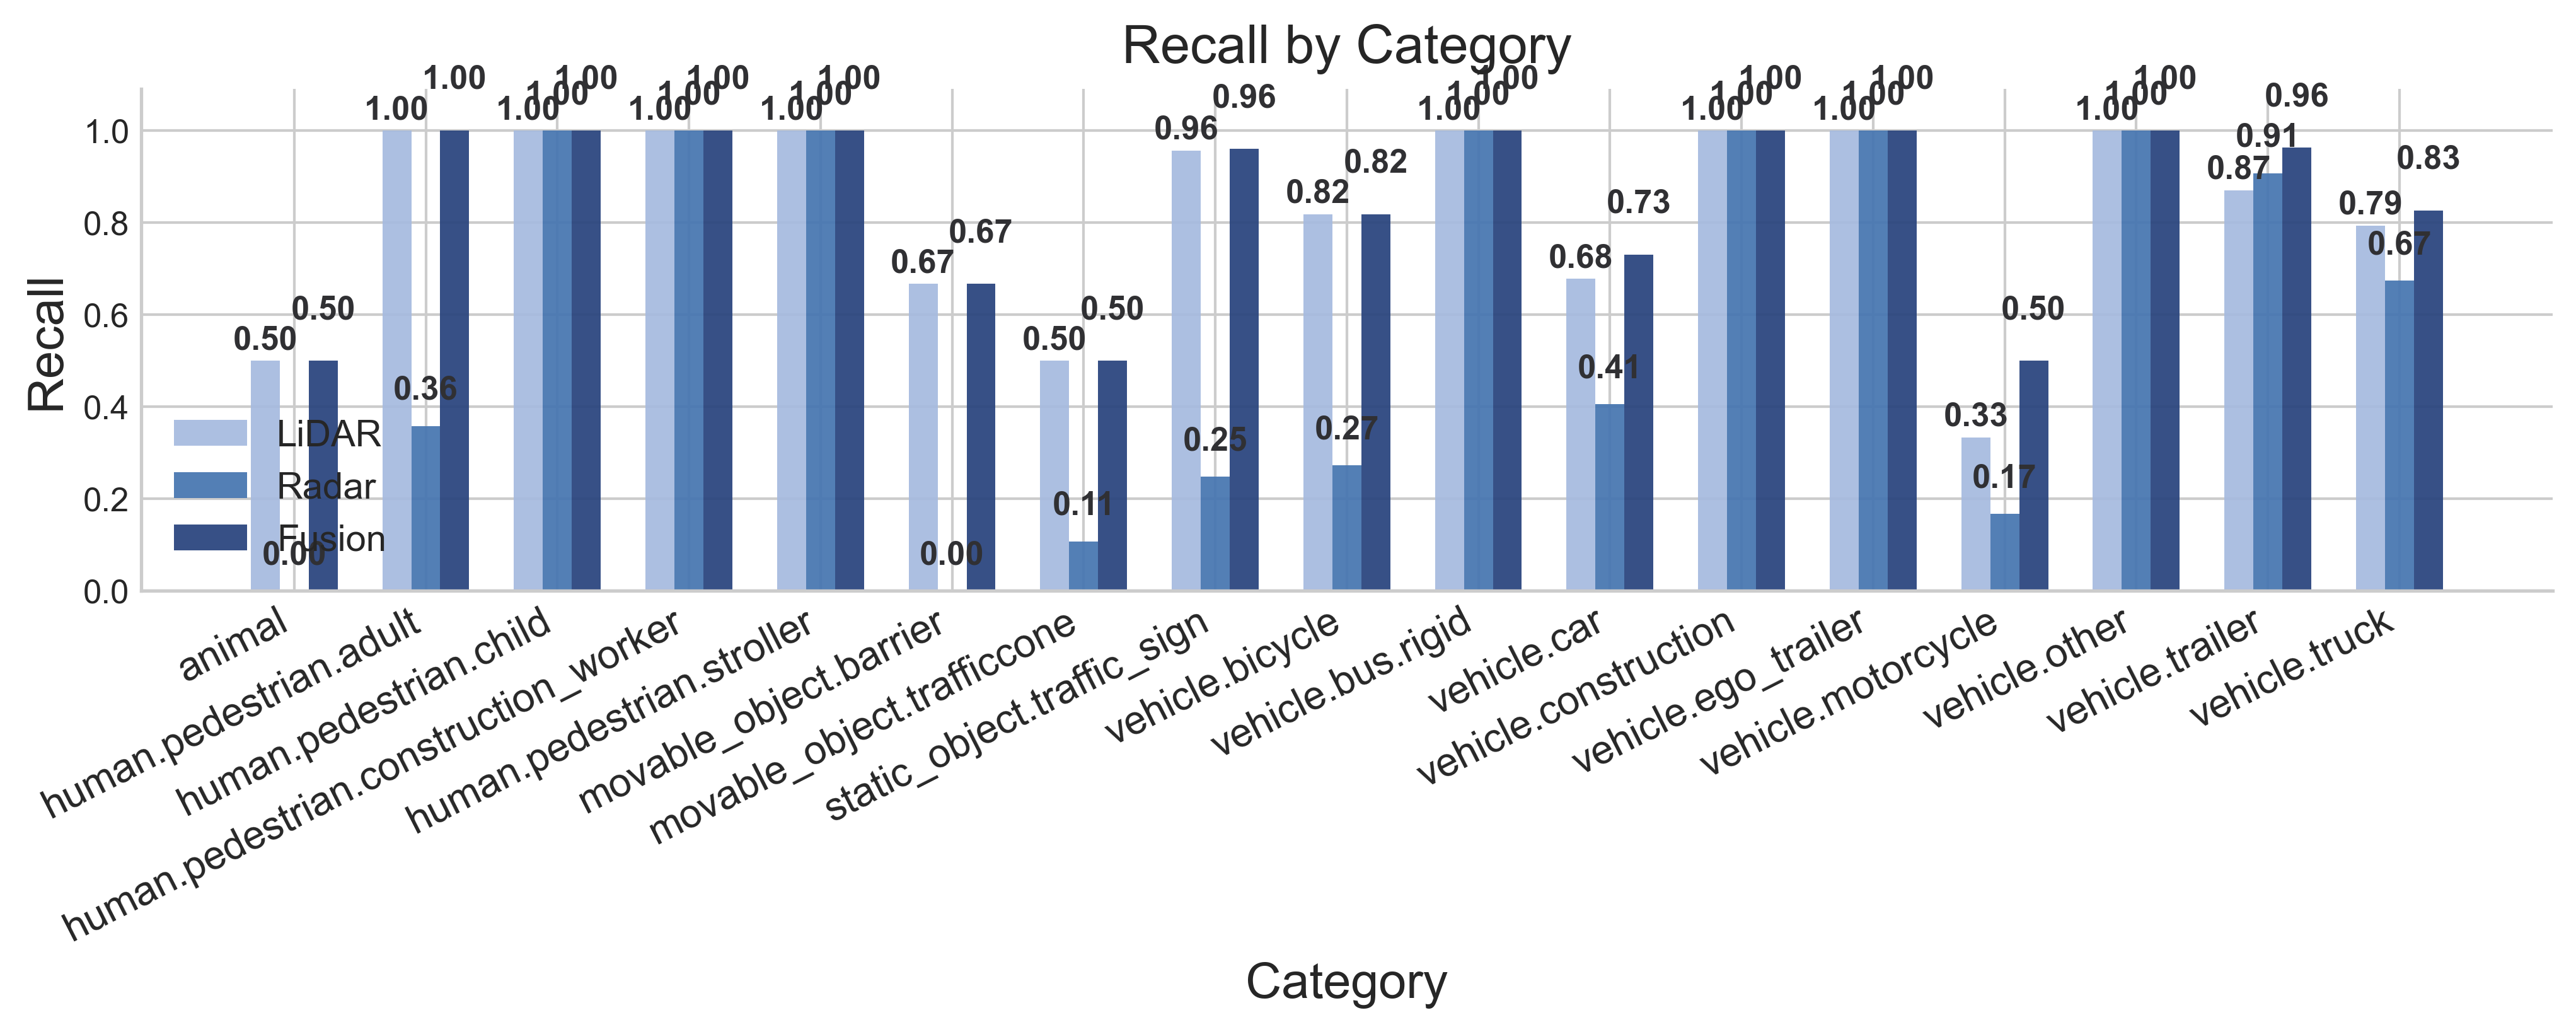
\includegraphics[width=0.7\textwidth]{../output/plots/recall_by_category.png}
    \caption{Recall by category.}
    \label{fig:recall_by_category}
\end{figure}

\begin{small}
% 中文:图\ref{fig:recall_by_category}展示了不同类别目标的recall。融合方案在大部分类别上均优于单一模态,尤其在人车等易漏检目标上提升明显,体现了多传感器互补优势。
\end{small}


\subsection{Performance Across Distance Ranges}
Figure~\ref{fig:recall_by_distance} presents recall as a function of object distance from the ego vehicle. It is evident that LiDAR and Radar alone exhibit a decline in detection recall at longer distances, whereas sensor fusion maintains higher recall across all distance bins. This highlights the enhanced robustness provided by multi-modal perception.

\begin{figure}[H]
    \centering
    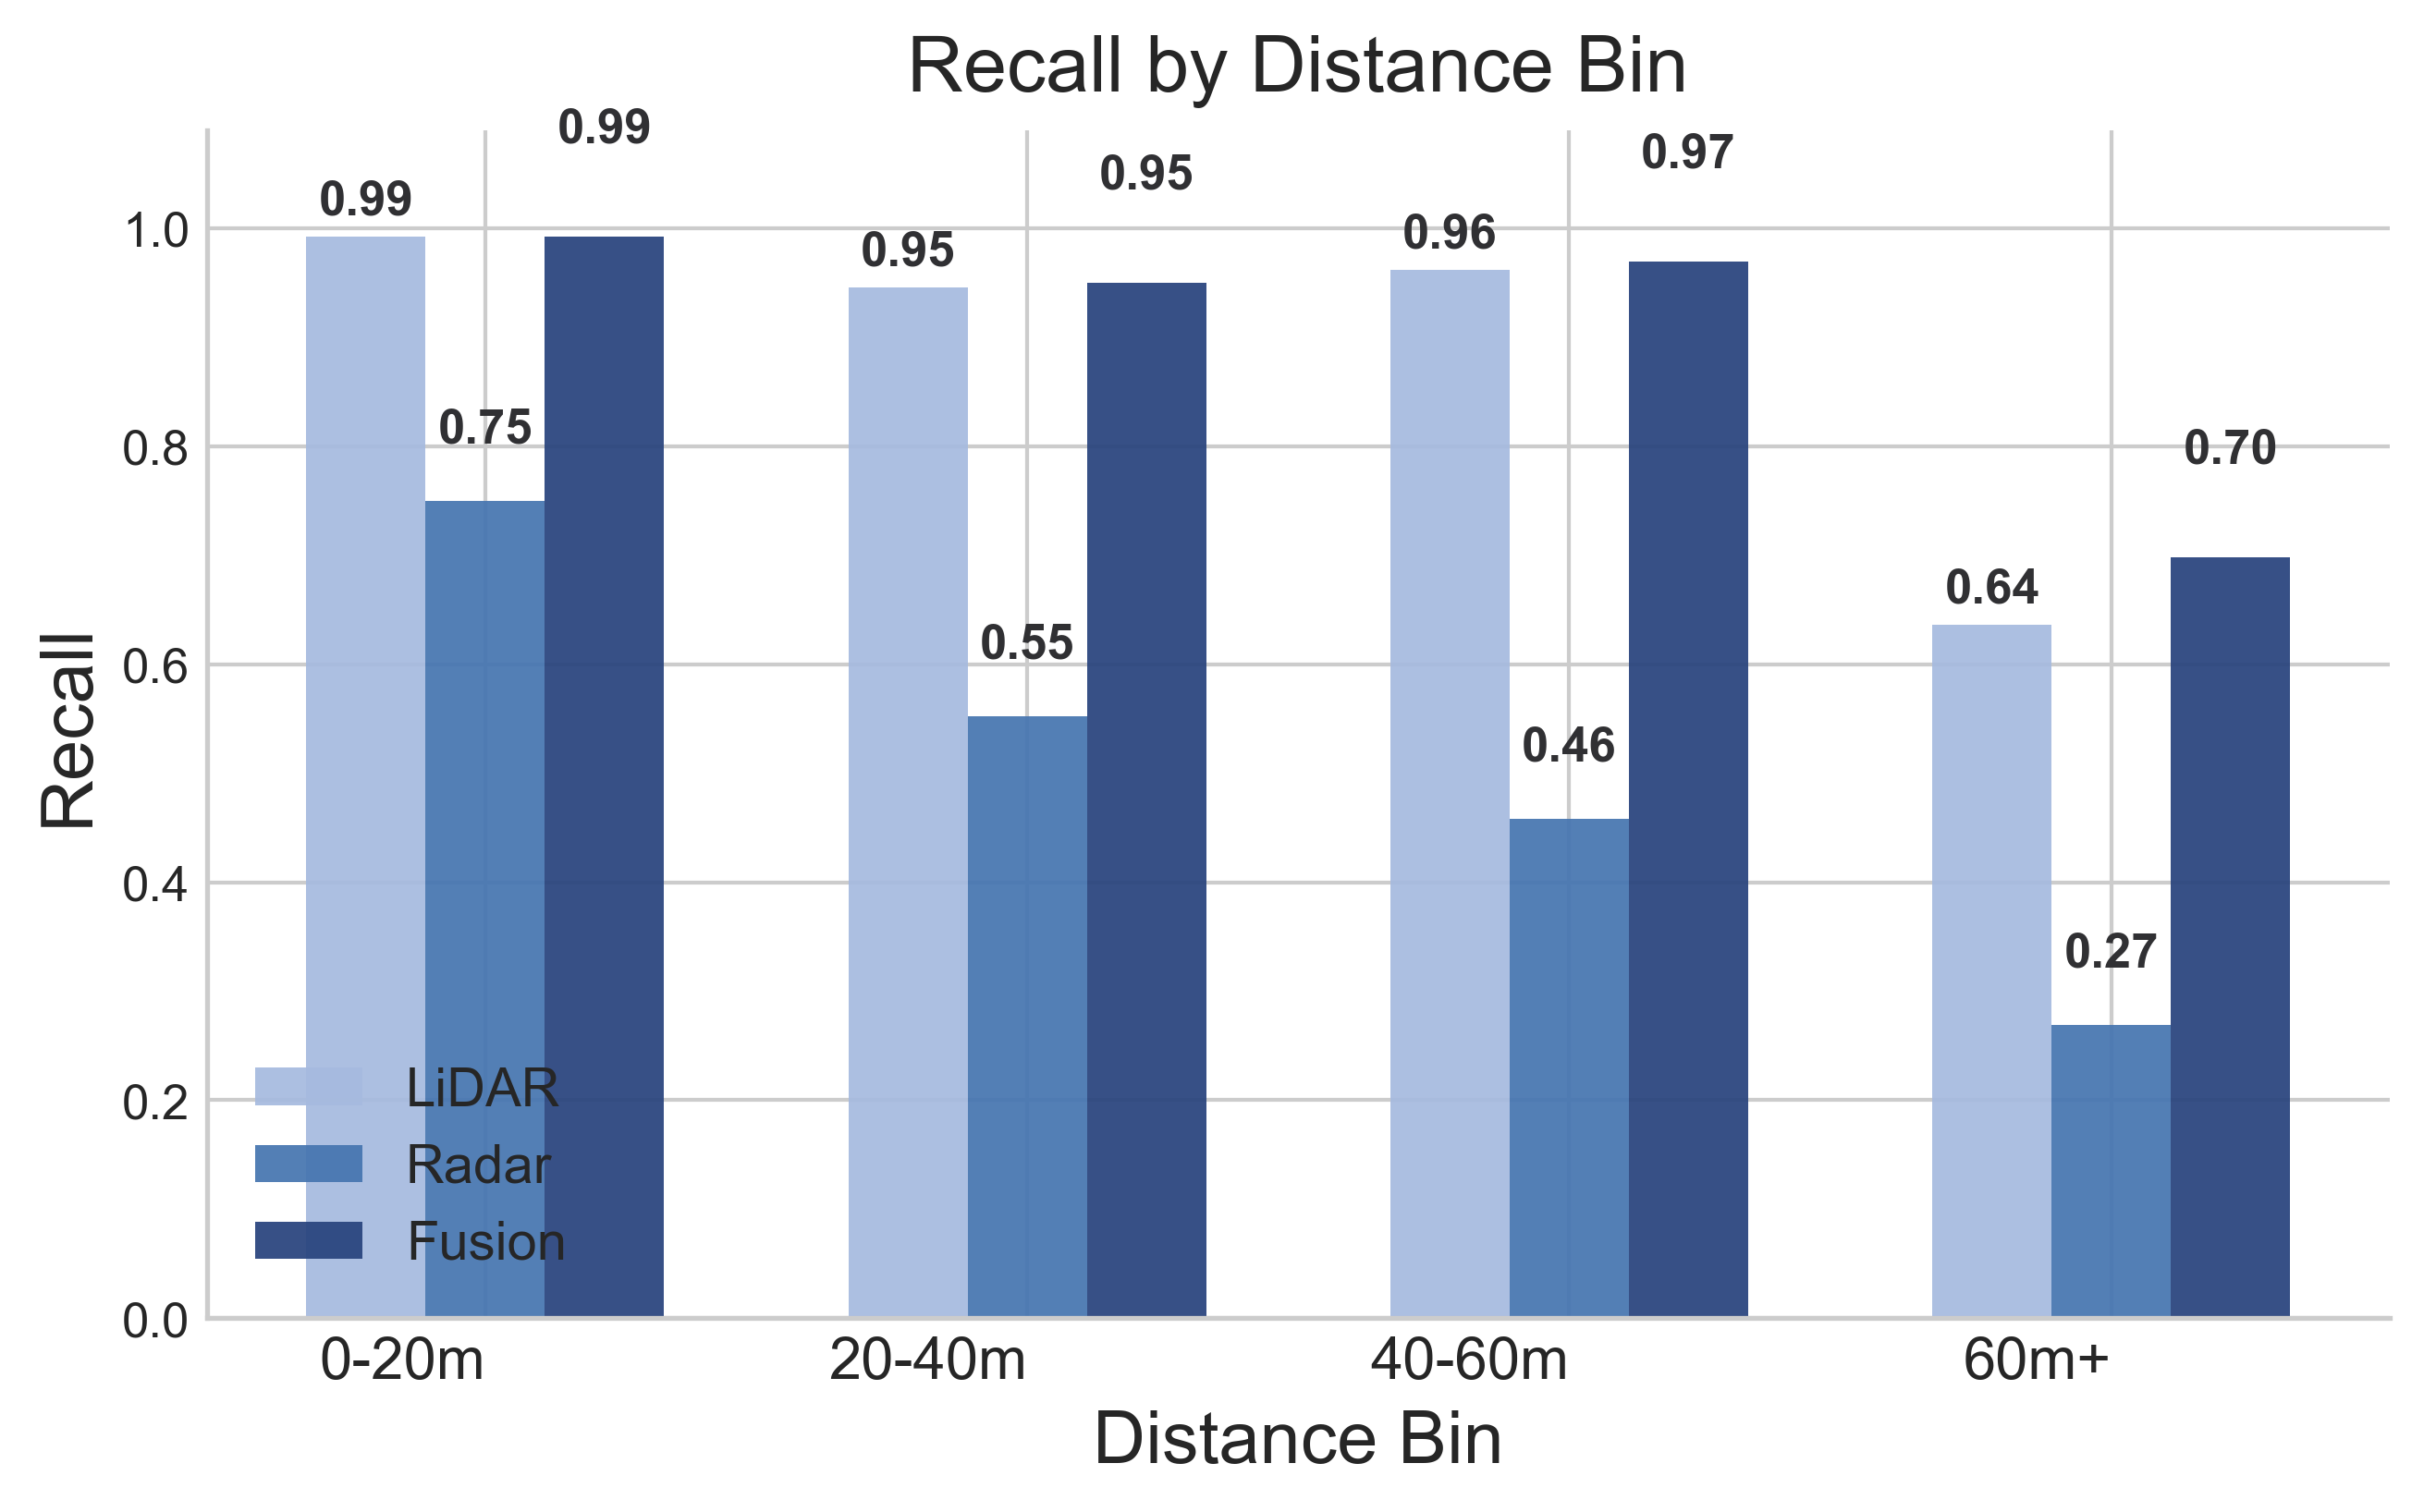
\includegraphics[width=0.5\textwidth]{../output/plots/recall_by_distance.png}
    \caption{Recall by distance range.}
    \label{fig:recall_by_distance}
\end{figure}

\begin{small}
%中文:图\ref{fig:recall_by_distance}展示了不同距离段的recall。随距离增加,单一传感器的检测率明显下降,而融合方案在各距离段均保持较高recall。这种远距离下的鲁棒性对于自动驾驶感知任务尤为关键。
\end{small}


\subsection{Summary of Findings}

Across all tested scenarios, categories, and ranges, sensor fusion is shown to provide more complete and robust detection coverage compared to any single modality. The automated pipeline enables reproducible, large-scale analysis and objective performance comparison under real-world conditions.

\begin{small}
% 中文:综合各场景、类别和距离分析,融合感知系统在目标检测完整性与鲁棒性上均明显优于单一传感器。所实现的自动化流程支持大规模、可复现实验及客观性能对比。
\end{small}


\section{Conclusion and Future Work}

In this work, a fully automated multi-sensor fusion pipeline has been developed and applied to large-scale autonomous driving perception analysis. LiDAR and Radar point clouds, originally recorded in their respective sensor frames, are precisely transformed into the ego-vehicle coordinate system through a series of calibration and pose operations. Three-dimensional object annotations are also converted from the global frame to the ego frame, ensuring spatial consistency for fusion, visualization, and quantitative analysis.

The implemented workflow supports batch processing and generates structured outputs, including recall statistics and multi-perspective visualizations, for nine representative scenarios. Experimental results demonstrate that sensor fusion significantly improves detection coverage and spatial alignment. This pipeline establishes a scalable and reproducible foundation for comprehensive evaluation of perception systems in real-world settings.

Potential future directions may include the integration of camera data and advanced deep learning-based fusion approaches, such as Transfuser, to further enhance perception robustness and enable end-to-end multi-modal learning.

\begin{small}
% 中文:本项目开发并应用了自动化多传感器融合感知分析流程,将LiDAR和Radar原始点云经标定与位姿变换精确对齐到自车坐标系,目标注释同样由全局系转为自车系,保证融合、可视化与统计分析的空间一致性。流程支持批量处理和结构化输出,覆盖九大典型场景。实验表明,融合方案在夜间高速、终端等复杂环境下显著提升了检测覆盖与空间对齐效果。该流程为真实驾驶场景下感知系统的综合评测建立了可扩展、可复现的基础。未来可探索引入相机数据与基于深度学习的Transfuser等方法,以进一步提升感知鲁棒性和多模态端到端能力。
\end{small}


\section*{References}
% 必要的参考文献(如MAN TruckScenes文档、论文等)
\begin{itemize}
    \item MAN TruckScenes Dataset and Devkit. \url{https://github.com/TUMFTM/truckscenes-devkit}
    \item ManTruck Official Documentation: \url{https://brandportal.man/d/QSf8mPdU5Hgj}
\end{itemize}
	
	
\end{document}